% chktex-file 1
\documentclass[
    10pt,
    oneside,   % symmetric pagination, for digital view
    a4paper,
    %english,
    italian
]{book}

\PassOptionsToPackage{dvipsnames}{xcolor} % colori PDF/A

\usepackage{colorprofiles}
% PDF/A
% validate in https://www.pdf-online.com/osa/validate.aspx
\usepackage[a-1a,mathxmp]{pdfx}[2018/12/22]
%\usepackage{amsmath,amssymb,amsthm} % matematica
\usepackage[T1]{fontenc}
\usepackage[utf8]{inputenc}
\usepackage[italian]{babel}
\usepackage{bookmark}
\usepackage{caption}
\usepackage{chngpage, calc} % centra il frontespizio
\usepackage{csquotes} % gestisce automaticamente i caratteri (")
\usepackage{emptypage} % pagine vuote senza testatina e piede di pagina
\usepackage{epigraph} % per epigrafi
%\usepackage{indentfirst} % rientra il primo paragrafo di ogni sezione
\usepackage{graphicx} % immagini
\usepackage[pdfa]{hyperref} % collegamenti ipertestuali
%\usepackage{hyperref}
\usepackage{listings} % codici
%\usepackage{microtype} % microtipografia
\usepackage{mparhack,relsize}  % finezze tipografiche
\usepackage{nameref} % visualizza nome dei riferimenti
\usepackage[font=small]{quoting} % citazioni
\usepackage{subfig} % sottofigure, sottotabelle
\usepackage[italian]{varioref} % riferimenti completi della pagina
\usepackage{booktabs} % tabelle
\usepackage{tabularx} % tabelle di larghezza prefissata
\usepackage{longtable} % tabelle su più pagine
\usepackage{ltxtable} % tabelle su più pagine e adattabili in larghezza
\usepackage[toc, acronym, automake]{glossaries}
\usepackage[backend=biber,style=verbose-ibid,hyperref,backref]{biblatex}
%\usepackage{layaureo} % margini ottimizzati per l'A4
\usepackage{lmodern}
\usepackage[left = 1in + 17pt + 0.6cm]{geometry} % Increased margins for single-page printing
\usepackage[inkscapelatex=false]{svg}
\usepackage{fancyhdr}
\usepackage{lipsum}
\usepackage{setspace}
\usepackage{titlesec}
\usepackage{rotating}
\geometry{a4paper, margin=1in}
\input{config/thesis-config}

\date{}

\hypersetup{pdfstartview=}
\begin{document}
    %\layout
    
    \frontmatter
    \input{preface/1_title-page}
    \input{preface/2_copyright}
    \cleardoublepage
\phantomsection
\pdfbookmark{Ringraziamenti}{Ringraziamenti}

%\begin{flushright}{
%    \slshape
%    ``I'm stronger, I'm smarter, I'm better''} \\
%    \medskip
%    --- Homelander.
%\end{flushright}
%
%\begin{flushright}{
%    \slshape
%    ``Non devo fuggire''} \\
%    \medskip
%    --- Shinji Ikari.
%\end{flushright}
%\begin{flushright}{
%    \slshape
%    ``Non dire gatto se non ce l'hai nel sacco''} \\
%    \medskip
%    --- Nonna.
%\end{flushright}
%\begin{flushright}{
%    \slshape
%    ``GG\textbackslash{}MM\textbackslash{}AAAAAAA''} \\
%    \medskip
%    --- Alex Scantamburlo.
%\end{flushright}
%
%\begin{flushright}{
%    \slshape
%    ``Ucciderò tutti i giganti''} \\
%    \medskip
%    --- Eren Yeager.
%\end{flushright}
%
%
%\begin{flushright}{
%    \slshape
%    ``Con il superamento della revisione PB -- a fronte di una prestazione estremamente deludente -- avete concluso il vostro progetto didattico di IS.''} \\
%    \medskip
%    --- Tullio Vardanega.
%\end{flushright}
%
%\begin{flushright}{
%    \slshape
%    ``Non posso aiutarvi''} \\
%    \medskip
%    --- Alessandro Staffolani.
%\end{flushright}
%
%\begin{flushright}{
%    \slshape
%    ``Mi avete fatto perdere mesi della mia vita''} \\
%    \medskip
%    --- Riccardo Cardin.
%\end{flushright}
%
%
%
\bigskip

\begingroup
\let\clearpage\relax
\let\cleardoublepage\relax
\let\cleardoublepage\relax

\chapter*{Ringraziamenti}
\emph{\noindent Innanzitutto, vorrei ringraziare il professor \myProf, relatore della tesi, per il sostegno e i consigli preziosi fornitomi durante la stesura del lavoro.}\\
\emph{Un ringraziamento va anche al tutor aziendale, \myCompanyTutor, per avermi seguito con attenzione e competenza durante l'esperienza di stage, e per avermi dato l'opportunità di lavorare su un progetto tanto stimolante quanto formativo.}\\
\emph{Desidero dedicare un ringraziamento speciale ai miei genitori, per avermi sempre sostenuto e incoraggiato, e per avermi permesso di intraprendere questo percorso di studi. Senza tale supporto, non avrei potuto raggiungere questo traguardo.}\\
\emph{Infine, vorrei ringraziare i miei amici, per aver condiviso con me le gioie e le fatiche di questi anni universitari.}\\
\bigskip


\noindent\textit{\myLocation, \myTime}
\hfill \myName

\endgroup

    \cleardoublepage
\phantomsection
\pdfbookmark{Compendio}{Compendio}
\begingroup
\let\clearpage\relax
\let\cleardoublepage\relax

\chapter*{Sommario}

Il presente documento descrive il lavoro svolto durante il periodo di stage svolta presso l'azienda \myCompany. Lo stage, svolto alla conclusione del percorso di studi triennale in Informatica presso l'Università degli Studi di Padova, ha avuto una durata complessiva di \myHours ore. L'obiettivo principale dello stage è stato quello di classificare e estrapolare informazioni contenute nelle mail PEC utilizzando i modelli di Machine Learning di AWS.

\endgroup
\vfill

    \input{preface/5_table-of-contents}
    \cleardoublepage
\phantomsection
%\pdfbookmark{}
\begingroup 
\let\clearpage\relax 
\let\cleardoublepage\relax 

\chapter*{Convenzioni tipografiche}
Riguardo la stesura del testo, relativamente al documento sono state adottate le seguenti convenzioni tipografiche:
\begin{itemize}
	\item gli acronimi, le abbreviazioni e i termini ambigui o di uso non comune menzionati vengono evidenziati in blu e definiti nel glossario, situato alla fine del presente documento;
	\item per la prima occorrenza dei termini riportati nel glossario viene utilizzata la seguente nomenclatura: \glsfirstoccur{<termine>};
	\item i termini in lingua straniera o facenti parti del gergo tecnico sono evidenziati con il carattere \emph{corsivo}.
\end{itemize}

\endgroup
\vfill

   % problema -  cosa hanno fatto gli altri - strumenti a disposizione - cosa ho fatto - cosa serve quello che ho fatto
    
    \cleardoublepage

    \mainmatter
    % chktex-file 2
% chktex-file 8
% chktex-file 11
% chktex-file 24
% chktex-file 26
\chapter{Introduzione}
\label{cap:introduzione}

%\begin{figure}[h!]
%    \centering
%    \includegraphics[width=1\columnwidth]{img/quantum_entanglement.png}
%    \caption{Lorem}
%    \label{fig:entanglement}
%\end{figure}
%
%Introduzione al contesto applicativo.
%
%Lorem Figure \ref{fig:entanglement}
%
%Esempio di utilizzo di un termine nel glossario \gls{api}.
%
%Esempio di citazione in linea
%\cite{site:agile-manifesto}.
%
%Esempio di citazione nel pie' di pagina
%citazione\footcite{womak:lean-thinking}
%
%Termine di glossario \gls{apig}
%
%\lipsum[1-2]


\section{L'azienda}

\myCompany è un'azienda italiana di sviluppo software e consulenza informatica. Da quarant'anni supporta la riorganizzazione dei processi in tutte le aree aziendali, progettando e realizzando soluzioni digitali integrate. 
\newline
L'azienda che ad oggi conta più di 600 dipendenti e oltre 2500 aziende seguite ha come sede principale Villa Ramanelli a Grisignano di Zocco, in provincia di Vicenza, poco distante dai Centri di Ricerca e Sviluppo (CRS) e dal Centro per la Formazione di Vicenza. Conta anche diverse filiati in Trentino-Alto Adige, Friuli-Venezia Giulia, Lombardia, Piemonte, Emilia-Romagna, Toscana, Campania e Puglia. 
\newline
L'azienda è organizata in Business Unit, dei centri di competenza specifici e autonomi ma in relazione costante. Ognuna delle quali è specializzata in un settore specifico. 
\newline
L'obiettivo principale è l'innovazione e il progresso tecnologico, con l'obiettivo di creare soluzioni software che siano in grado di rispondere alle esigenze dei clienti, garantendo la massima qualità e sicurezza.
\newline
La metodologia di lavoro, indipendentemente dalla Business Unit, è basata su un approccio Agile implementata con il framework Scrum. Agile è un approccio alla gestione dei progetti che si basa su principi di collaborazione, auto-organizzazione e flessibilità. Scrum è un framework Agile che permette di gestire progetti complessi, garantendo la massima trasparenza e la massima flessibilità.
\newline
Ulteriori informazioni sono disponibili sul sito web dell'azienda\footnote{\url{https://www.sanmarcoinformatica.com/}}.
\begin{figure}[h!]
    \centering
    
\includegraphics[width=0.5\columnwidth]{img/logo_sanmarco_informatica.png}
    \caption{Logo di Sanmarco Informatica}
    \label{fig:entanglement}
\end{figure}
\section{L'offerta di stage}
L'idea dello stage consiste nella catalogazione delle Poste Elettroniche Certificate (PEC) integrando tecnologie di Intelligenza Artificiale (AI) per l'analisi e l'efficienza del processo. 
\newline
Il modello di apprendimento automatico analizza il contenuto delle PEC e le classifica in base al contenuto. 
\newline
Il progetto è stato proposto dall'azienda in occasione dell'evento Stage IT 2024, organizzato dall'Università degli Studi di Padova e promosso da Confindustria Veneto Est. Tale evento mira ad agevolare l'incontro tra studenti e aziende, offrendo la possibilità di svolgere uno stage formativo con specifico riferimento al settore ICT.

\section{Organizzazione del testo}

\begin{description}
    \item[{\hyperref[cap:processi-metodologie]{Il secondo capitolo}}] descrive ...
    
    \item[{\hyperref[cap:descrizione-stage]{Il terzo capitolo}}] approfondisce ...
    
    \item[{\hyperref[cap:analisi-requisiti]{Il quarto capitolo}}] approfondisce ...
    
    \item[{\hyperref[cap:progettazione-codifica]{Il quinto capitolo}}] approfondisce ...
    
    \item[{\hyperref[cap:verifica-validazione]{Il sesto capitolo}}] approfondisce ...
    
    \item[{\hyperref[cap:conclusioni]{Nel settimo capitolo}}] descrive ...
\end{description}

Riguardo la stesura del testo, relativamente al documento sono state adottate le seguenti convenzioni tipografiche:
\begin{itemize}
	\item gli acronimi, le abbreviazioni e i termini ambigui o di uso non comune menzionati vengono definiti nel glossario, situato alla fine del presente documento;
	%\item per la prima occorrenza dei termini riportati nel glossario viene utilizzata la seguente nomenclatura: \emph{parola}\glsfirstoccur;
	\item i termini in lingua straniera o facenti parti del gergo tecnico sono evidenziati con il carattere \emph{corsivo}.
\end{itemize}

    % chktex-file 24

\chapter{Descrizione dello stage}
\label{cap:descrizione-stage}

\emph{In questo capitolo}
%\intro{Breve introduzione al capitolo}\\

\section{Introduzione al progetto}

L'elaborazione intelligente dei documenti (\glsfirstoccur{\gls{idpg}}) è una tecnologia che automatizza il processo di immissione manuale dei dati da documenti cartacei o immagini digitali, integrandoli con altri processi aziendali digitali. Ad esempio, in un flusso di lavoro aziendale automatizzato, come l'invio di ordini ai fornitori al momento del calo delle scorte, l'\gls{idpg} può sostituire l'immissione manuale dei dati da parte del team contabile. Invece di inserire manualmente i dati di una fattura ricevuta via e-mail, i sistemi di \gls{idpg} estraggono automaticamente queste informazioni e le integrano direttamente nel sistema contabile, eliminando ostacoli e riducendo gli errori.

L'\gls{idpg} offre numerosi vantaggi alle aziende. In termini di \glsfirstoccur{\gls{scalabilitàg}}, permette di elaborare documenti su larga scala con precisione, evitando errori umani e aumentando l'efficienza operativa. Promuove una **cultura dell’efficienza dei costi**, automatizzando attività ripetitive e riducendo i costi associati all'elaborazione manuale dei dati. Migliora anche la **soddisfazione dei clienti** grazie alla gestione più rapida e automatizzata dei documenti, come l'onboarding, le prenotazioni e i pagamenti, consentendo di fornire risposte personalizzate e veloci ai clienti.

Diversi settori traggono beneficio dall'\gls{idpg}. Nel **settore sanitario**, facilita la gestione delle cartelle cliniche, migliorando l'estrazione e l'organizzazione dei dati dai documenti medici. Le **aziende finanziarie** lo utilizzano per automatizzare la gestione delle spese e l'elaborazione delle fatture, semplificando la gestione dei pagamenti. Nel **settore legale**, l'\gls{idpg} analizza contratti e documenti legali, utilizzando tecnologie di elaborazione del linguaggio naturale (\glsfirstoccur{\gls{nlpg}}) per estrarre informazioni chiave. Le aziende della **logistica** lo impiegano per tracciare spedizioni e documenti di transito, riducendo gli errori umani. Infine, nel settore delle **risorse umane**, l'\gls{idpg} semplifica la selezione del personale, gestisce le buste paga e automatizza altre funzioni HR.

Le tecnologie alla base dell'\gls{idpg} comprendono il **riconoscimento ottico dei caratteri (\glsfirstoccur{\gls{ocrg}})**, che converte immagini di testo in dati leggibili dalle macchine, e l'**elaborazione del linguaggio naturale (\gls{nlpg})**, che analizza e comprende il linguaggio umano. L'**automazione robotica dei processi (RPA)** consente invece di automatizzare i flussi di lavoro aziendali ripetendo azioni umane predefinite.

Il processo di IDP si articola in diverse fasi: acquisizione e **classificazione dei documenti**, **estrazione dei dati** rilevanti tramite \gls{ocrg} e \gls{nlpg}, **convalida e successiva elaborazione dei dati** nei sistemi aziendali, e **apprendimento continuo** attraverso algoritmi di machine learning per migliorare l'accuratezza nel tempo. Inoltre, i sistemi di \gls{idpg} offrono **report e analisi** per ottimizzare ulteriormente i flussi di lavoro aziendali.

\glsfirstoccur{\gls{awsg}} (AWS) supporta l'implementazione dell'\gls{idpg} attraverso servizi come **Amazon Textract**, che utilizza il machine learning per estrarre informazioni dai documenti senza interazioni manuali, e **Amazon Comprehend**, che sfrutta l'\gls{nlpg} per scoprire informazioni preziose nei testi. Entrambi i servizi consentono alle aziende di automatizzare la gestione dei documenti in modo efficiente e sicuro, integrandosi con altre piattaforme aziendali per un flusso di lavoro senza interruzioni.

%\begin{figure}[!ht]
%    \centering
%    \includegraphics[width=0.5\columnwidth]{pk_estate.jpg}
%    \caption{Caption}
%\end{figure}
%Digressione su idp.\\
%\lipsum[1]

%\section{Analisi preventiva dei rischi}
%
%Durante la fase di analisi iniziale sono stati individuati alcuni possibili
%rischi a cui si potrà andare incontro. Si è quindi proceduto a elaborare delle
%possibili soluzioni per far fronte a tali rischi.
%
%\begin{risk}{Performance del simulatore hardware}
%    \riskdescription{le performance del simulatore hardware e la comunicazione con questo potrebbero risultare lenti o non abbastanza buoni da causare il fallimento dei test}
%    \risksolution{coinvolgimento del responsabile a capo del progetto relativo il simulatore hardware}
%    \label{risk:hardware-simulator}
%\end{risk}
%
\section{Requisiti e obiettivi}
Gli obiettivi sono stati definiti in accordo con il tutor aziendale e si
identificano nel seguente modo:
\[
    \text{[Priorità][Id]}
\]
\begin{itemize}
    \item Priorità: indica la priorità dell'obiettivo, può essere obbligatorio o
          desiderabile;
    \item Id: composto da due cifre, identifica l'obiettivo in modo univoco rispetto alla priorità.
\end{itemize}

\begin{longtable}{|c|p{4cm}|p{10cm}|}
    \hline
    \textbf{ID}  & \textbf{Categoria}                                               & \textbf{Descrizione}                                       \\
    \hline
    \endfirsthead

    \hline
    \textbf{ID}  & \textbf{Categoria}                                               & \textbf{Descrizione}                                       \\
    \hline
    \endhead

    O01          & Obbligatorio                                                     & Analisi dei servizi \gls{awsg} per l'addestramento dei modelli \gls{aig}
    \\ \hline O02 & Obbligatorio & Addestramento di un modello di apprendimento \gls{aig}
    utilizzando i servizi \gls{awsg}                                                                                                                    \\ \hline O03 & Obbligatorio & Analisi requisiti
    applicativi e tecnici per implementare la soluzione richiesta                                                                                \\ \hline O04   &
    Obbligatorio & Implementare un modello di apprendimento automatico che analizzi
       il contenuto delle \gls{pecg} importate e assegni loro categorie appropriate in base
    al contenuto (mittente, destinatario, data e argomento)                                                                                      \\ \hline D01   &
    Desiderabile & Implementare algoritmi di \gls{aig} in grado di adattarsi e apprendere
       continuamente dai dati per migliorare le prestazioni del sistema nel tempo. Ciò
       include l'ottimizzazione dei modelli di apprendimento automatico in base
    all'esperienza e ai feedback degli utenti                                                                                                    \\ \hline D02 & Desiderabile &
       Integrazione con un sistema documentale per l’archiviazione delle \gls{pecg} creando i
       metadati necessari con le informazioni estratte e collocandole nella corretta
    categoria di appartenenza                                                                                                                    \\ \hline
\end{longtable}

\section{Pianificazione}
\subsection{Pianificazione settimanale}
Il periodo di stage è stato suddiviso in 8 settimane, durante le quali sono
previste le seguenti attività:
\begin{longtable}{|c|c|c|p{8cm}|}
    \hline
    \textbf{Settimana} & \textbf{Dal} & \textbf{Al} & \textbf{Attività}                                          \\
    \hline
    \endfirsthead

    \hline
    \textbf{Settimana} & \textbf{Dal} & \textbf{Al} & \textbf{Attività}                                          \\
    \hline
    \endhead

    1                  & 24-06-2024   & 28-06-2024  &
    - Incontro con persone coinvolte nel progetto per discutere i requisiti e le richieste di implementazione \newline
    - Ricerca, studio e documentazione per inquadramento progetto \newline
    - Introduzione ai linguaggi di sviluppo \newline
    - Introduzione agli ambienti di sviluppo \newline
    - Introduzione dei servizi \gls{awsg}                                                                       \\
    \hline
    2                  & 01-07-2024   & 05-07-2024  &
    - Analisi dei servizi \gls{awsg} per l'addestramento di un modello di apprendimento \newline
    - Addestramento di un modello di apprendimento utilizzando i servizi di \gls{awsg} \newline
    \textbf{Milestone:} Utilizzo dei servizi \gls{awsg} per l'addestramento di un modello di apprendimento              \\
    \hline
    3                  & 08-07-2024   & 12-07-2024  &
    - Studio della soluzione per definire i requisiti necessari per l’implementazione \newline
    \textbf{Milestone:} Analisi dei requisiti applicativi e tecnici per implementare la soluzione                \\
    \hline
    4                  & 15-07-2024   & 19-07-2024  &
    - Addestramento modello di apprendimento per catalogare le \gls{pecg} in base al loro contenuto                     \\
    \hline
    5                  & 22-07-2024   & 26-07-2024  &
    - Implementazioni per interfacciarsi con il modello di apprendimento addestrato e per poter catalogare le \gls{pecg} importate \newline
    \textbf{Milestone:} Completamento obiettivi minimi                                                           \\
    \hline
    6                  & 29-07-2024   & 02-08-2024  &
    - Implementazione algoritmo di \gls{aig} per l’autoapprendimento                                                    \\
    \hline
    7                  & 05-08-2024   & 09-08-2024  &
    - Studio e documentazione sulle \gls{apig} messe a disposizione dal documentale per poter catalogare le mail \gls{pecg} \newline
    - Implementazione dell’integrazione con il documentale producendo i metadati necessari per catalogare le \gls{pecg} \\
    \hline
    8                  & 12-08-2024   & 16-08-2024  &
    - Verifica e test archiviazione \gls{pecg} nel documentale \newline
    \textbf{Milestone:} Completamento obiettivi massimi                                                          \\
    \hline
    9                  & 19-08-2024   & 23-08-2024  &
    - Recupero eventuali ritardi                                                                                 \\
    \hline
    10                 & 26-08-2024   & 30-08-2024  &
    - Recupero eventuali ritardi                                                                                 \\
    \hline

\end{longtable}
    \chapter{Tecnologie e strumenti di interesse}
\label{cap:tecnologie}
\emph{In questo capitolo verranno descritti i servizi e le tecnologie analizzate e pertinenti per il problema descritto, in quale modo possono essere impiegate e una panoramica finalizzata a chiarirne il contesto e il caso d'uso.}

\section{Amazon Web Services}
\gls{aws} è una piattaforma di servizi cloud che offre potenza di calcolo, storage di database, distribuzione di contenuti e altre funzionalità per aiutare le aziende a scalare e crescere. AWS offre una vasta gamma di servizi che possono essere utilizzati per implementare soluzioni di \gls{ai} e \gls{mlg} e in particolare che possano implementare un flusso di \gls{idpg} automatizzato e adatto agli obiettivi del progetto.\\
Per la realizzazione dell'applicazione sono stati individuati diversi servizi che hanno permesso di realizzare un'architettura scalabile e \gls{serverlessg}.

\subsection{Amazon Comprehend}
Amazon Comprehend (il logo è riportato in Figura \ref{fig:comprehend}) è un servizio avanzato di analisi del linguaggio naturale (\gls{nlpg}) che utilizza algoritmi di apprendimento automatico per estrarre informazioni significative dai testi. Il servizio è in grado di identificare entità, frasi chiave, lingua, sentimenti e altre caratteristiche comuni all'interno dei documenti, offrendo la possibilità di effettuare analisi sia in tempo reale che in modalità asincrona su grandi volumi di dati. Gli utenti possono scegliere di utilizzare modelli pre-addestrati o di addestrare modelli personalizzati per specifiche esigenze di classificazione e riconoscimento delle entità.\\
Tra le principali funzionalità di Amazon Comprehend vi è \textit{Amazon Comprehend Insights}, che consente di analizzare documenti, singoli o in gruppo, per identificare le informazioni più rilevanti utilizzando modelli già addestrati. Questi modelli possono essere impiegati per individuare entità (come persone, luoghi, date, quantità, ecc.), frasi chiave, informazioni personali identificabili, 
sentiment (positivo, negativo, neutro) oltre a determinare la lingua e la sintassi del testo.\\
Un'altra funzionalità rilevante è \textit{Amazon Comprehend Custom}, che permette la creazione di modelli \gls{nlpg} personalizzati per la classificazione (\textit{Custom Classification}) e il riconoscimento delle entità (\textit{Custom Entity Recognition}). La \textit{Custom Classification} consente di categorizzare i documenti in base a categorie predefinite, mentre la \textit{Custom Entity Recognition} permette di individuare entità specifiche all'interno dei testi. Entrambi i servizi richiedono una fase di training che necessita di un \glsfirstoccur{\gls{datasetg}} etichettato per addestrare il modello e supportano l'elaborazione dei documenti in un'unica fase.\\
In aggiunta, Amazon Comprehend offre la funzionalità \textit{Flywheel}, che semplifica il processo di addestramento e gestione delle versioni dei modelli personalizzati, facilitando l'orchestrazione delle attività di training, valutazione e deployment dei modelli. Consiste dunque nel riferimento principale per la fase di \glsfirstoccur{\gls{mlops}} e permette di monitorare le prestazioni dei modelli, valutare le metriche di accuratezza e precisione e gestire le versioni dei modelli in produzione.\\
Infine, il \textit{Document Clustering} permette di raggruppare i documenti in base a parole chiave ricorrenti, rendendo più agevole l'identificazione di documenti simili e la loro organizzazione per categorie o argomenti.\\
Nel presente lavoro, Amazon Comprehend è stato utilizzato per la classificazione dei documenti nelle categorie selezionate tramite la funzionalità \textit{Custom Classification}.

\begin{figure}[h]
  \centering
  
\includegraphics[width=0.2\textwidth]{img/tecnologie/comprehend.png}
  \caption{Logo di Amazon Comprehend}
  \label{fig:comprehend}
\end{figure}

\subsection{Amazon Textract}
Amazon Textract (il logo è riportato in Figura \ref{fig:textract}) è un servizio di riconoscimento ottico dei caratteri (\gls{ocr}) che sfrutta l'apprendimento automatico per identificare e analizzare testo e dati presenti in immagini o documenti. Basato sulla tecnologia di \glsfirstoccur{\gls{deeplearningg}} collaudata e altamente scalabile sviluppata dagli esperti di \glsfirstoccur{\gls{computervisiong}} di Amazon, Textract è in grado di analizzare quotidianamente miliardi di immagini e video. Una delle caratteristiche distintive di questo servizio è la sua accessibilità: non è richiesta alcuna esperienza nel campo del \gls{ml} per utilizzarlo, grazie alla disponibilità di \gls{apig} semplici e intuitive che consentono di analizzare file immagine e PDF con facilità. Inoltre, Amazon Textract apprende continuamente dai nuovi dati e Amazon implementa costantemente nuove funzionalità, garantendo un miglioramento continuo delle sue capacità.

Il servizio non si limita a eseguire il riconoscimento ottico dei caratteri da testo digitato o scritto a mano, ma è anche in grado di estrarre il contenuto del documento, incluse tabelle, campi e relazioni strutturali. Textract fornisce punteggi di confidenza e bounding box (rappresentazioni grafiche dei confini) per ogni parola e riga di testo riconosciuta. Il servizio supporta vari formati di file, tra cui PDF, TXT, DOC, DOCX, JPG e PNG.

Le principali funzionalità di Amazon Textract includono:

\begin{itemize}
    \item \textbf{Estrazione di testo non strutturato}: Questa funzionalità consente di estrarre i dati in forma di parole (\textit{WORDS}) e righe di testo (\textit{LINES}), senza mantenere la formattazione originaria del documento. Per questa operazione si utilizza l'\gls{apig} \texttt{DetectDocumentText}.
    
    \item \textbf{Estrazione ed elaborazione di moduli e tabelle}: Tramite l'\gls{apig} \texttt{AnalyzeDocument}, è possibile estrarre dati mantenendo la struttura del documento originale, identificando parole, righe, tabelle e moduli (\textit{WORDS}, \textit{LINES}, \textit{TABLES}, \textit{FORMS}).
    
    \item \textbf{Estrazione di coppie chiave-valore}: Utilizzando l'\gls{apig} \texttt{AnalyzeDocument}, questa funzionalità permette di estrarre informazioni strutturate in forma di chiavi e valori, preservando la formattazione del documento.
    
    \item \textbf{Estrazione tramite query}: Questa funzionalità consente di focalizzarsi su informazioni specifiche o critiche all'interno di un documento. Anche in questo caso, l'\gls{apig} utilizzata è \texttt{AnalyzeDocument}.
    
    \item \textbf{Rilevamento delle firme}: Attraverso l'\gls{apig} \texttt{AnalyzeDocument}, è possibile rilevare la presenza di firme nei documenti, restituendo un punteggio di confidenza per il rilevamento, oltre al testo del documento in forma di parole e righe (\textit{WORDS} e \textit{LINES}).
    
    \item \textbf{Estrazione di informazioni da fatture e ricevute}: L'\gls{apig} \texttt{AnalyzeExpense} è specificamente progettata per estrarre dati da documenti contabili come fatture e ricevute.
    
    \item \textbf{Estrazione di informazioni da documenti di identità}: Utilizzando l'\gls{apig} \texttt{AnalyzeID}, è possibile estrarre dati rilevanti da documenti di identità.
    
    \item \textbf{Rilevamento di testo su più colonne}: Questa funzionalità consente di riconoscere e trattare testi distribuiti su più colonne all'interno di un documento.
\end{itemize}

Per migliorare la precisione delle analisi e ridurre l'intervento umano necessario, Amazon Textract offre lo strumento delle \textit{Custom Queries}. Questo strumento consente di riconoscere specifici termini univoci, strutture particolari e informazioni specifiche all'interno dei documenti, offrendo un livello di personalizzazione superiore rispetto alle query standard.

Un'altra opzione avanzata per personalizzare l'output dell'analisi dei documenti è l'uso degli \textit{Adapters}. Gli Adapters sono componenti che si integrano nel modello di \gls{deeplearningg} pre-addestrato di Amazon Textract, permettendo di personalizzare l'output in base ai documenti specifici di un'azienda. Per creare un Adapter, è necessario annotare ed etichettare un insieme di documenti campione e addestrare l'Adapter su questi campioni annotati.

Una volta creato un Adapter, Amazon Textract fornisce un \textit{AdapterId}. È possibile creare e gestire diverse versioni di un Adapter all'interno di uno stesso identificatore. L'\textit{AdapterId}, insieme alla versione dell'Adapter, può essere utilizzato in una richiesta per specificare l'uso dell'Adapter creato durante l'analisi dei documenti. Ad esempio, questi parametri possono essere forniti all'\gls{apig} \texttt{AnalyzeDocument} per un'analisi sincrona dei documenti, oppure all'operazione \texttt{StartDocumentAnalysis} per un'analisi asincrona. Includendo l'\textit{AdapterId} nella richiesta, l'Adapter verrà automaticamente integrato nel processo di analisi, migliorando le previsioni per i documenti specifici.

Questo approccio consente di sfruttare le capacità dell'\gls{apig} \texttt{AnalyzeDocument} mentre si adatta il modello alle esigenze specifiche del proprio caso d'uso. 

Nel contesto del presente lavoro, Amazon Textract è stato utilizzato per estrarre il testo dai documenti sia come input al classificatore di Comprehend sia per estrarre informazioni utili.

\begin{figure}[h]
  \centering
  
\includegraphics[width=0.2\textwidth]{img/tecnologie/textract.png}
  \caption{Logo di Amazon Textract}
  \label{fig:textract}
\end{figure}

\subsection{Amazon S3}
Amazon Simple Storage Service (Amazon S3) (logo riportato in Figura \ref{fig:s3}) è un servizio di storage di oggetti che offre elevata scalabilità, disponibilità dei dati, sicurezza e prestazioni. Amazon S3 è progettato per gestire grandi volumi di dati a costi contenuti, risultando una soluzione ideale per applicazioni che richiedono capacità di archiviazione massiva.

Per memorizzare dati in Amazon S3, è necessario utilizzare un \textit{bucket}, che funge da contenitore per gli oggetti. Ogni oggetto in un \textit{bucket} rappresenta un file e i relativi metadati associati. La procedura per archiviare un oggetto in Amazon S3 prevede la creazione di un \textit{bucket} e il successivo caricamento dell'oggetto al suo interno. Una volta caricato, l'oggetto può essere aperto, scaricato o eliminato. Qualora un oggetto o un \textit{bucket} non siano più necessari, è possibile procedere alla loro eliminazione.

Nel contesto del presente progetto, Amazon S3 è stato utilizzato per memorizzare i file relativi alle diverse fasi del lavoro, inclusi allegati, email, file CSV impiegati per l'addestramento dei modelli e file di output generati dalle analisi. 


\begin{figure}[h]
  \centering
  
\includegraphics[width=0.2\textwidth]{img/tecnologie/s3.png}
  \caption{Logo di Amazon S3}
  \label{fig:s3}
\end{figure}

\subsection{AWS Lambda}
AWS Lambda (logo riportato in Figura \ref{fig:lambda}) è un servizio di calcolo \gls{serverlessg} che esegue codice in risposta a eventi, gestendo automaticamente le risorse di calcolo necessarie. Questo servizio elimina la necessità di provisioning e gestione dei server, offrendo una soluzione scalabile e affidabile per diverse applicazioni.

Il codice in Lambda è organizzato in funzioni che vengono eseguite solo quando richiesto, scalando automaticamente in base al carico. La tariffazione si basa esclusivamente sul tempo di calcolo utilizzato, senza costi aggiuntivi quando il codice non è in esecuzione. Questa flessibilità lo rende ideale per scenari che richiedono scalabilità dinamica e riduzione automatica delle risorse in assenza di carico.

Nel contesto del presente progetto, AWS Lambda è stato impiegato per implementare le funzioni di chiamate \gls{apig}, garantendo un'architettura serverless efficiente. Le funzioni Lambda sono state integrate con altri servizi AWS, come Amazon S3 per l'elaborazione dei file e Amazon API Gateway per la gestione delle richieste \gls{apig}. L'adozione di Lambda ha permesso di semplificare la gestione operativa, poiché il servizio si occupa automaticamente di capacità, monitoraggio e logging, lasciando agli sviluppatori la responsabilità esclusiva del codice.


\begin{figure}[h]
  \centering
  
\includegraphics[width=0.3\textwidth]{img/tecnologie/AWS_Lambda.png}
  \caption{Logo di AWS Lambda}
  \label{fig:lambda}
\end{figure}

\subsection{Amazon DynamoDB}
Amazon DynamoDB (logo riportato in Figura \ref{fig:dynamodb}) è un servizio di database \glsfirstoccur{\gls{nosqlg}} completamente gestito, progettato per garantire prestazioni a singola cifra di millisecondi indipendentemente dalla scala. Ideale per carichi di lavoro operativi che richiedono alta efficienza, DynamoDB affronta le complessità di scalabilità e gestione operativa tipiche dei database relazionali, mantenendo prestazioni elevate anche in presenza di un grande numero di utenti. Questo lo rende particolarmente adatto per applicazioni moderne che necessitano di crescere rapidamente a livello globale.

Dal suo lancio nel 2012, DynamoDB è stato adottato da organizzazioni di ogni settore e dimensione per sviluppare applicazioni che possono iniziare con piccoli volumi di dati e scalare fino a supportare tabelle di dimensioni virtualmente illimitate, assicurando al contempo alta disponibilità.

Nel contesto del presente progetto, Amazon DynamoDB è stato utilizzato per la memorizzazione dei dati estratti dai documenti e delle classificazioni effettuate, garantendo un accesso rapido e affidabile alle informazioni archiviate.



\begin{figure}[h]
  \centering
  
\includegraphics[width=0.3\textwidth]{img/tecnologie/DynamoDB.png}
  \caption{Logo di Amazon DynamoDB}
  \label{fig:dynamodb}
\end{figure}
\subsection{AWS Step Functions}
AWS Step Functions (logo riportato in Figura \ref{fig:stepfunctions}) è un servizio di orchestrazione \gls{serverlessg} che consente di coordinare in modo efficiente i componenti di applicazioni distribuite, microservizi e pipeline di dati o di \gls{mlg} attraverso una logica visuale. Questo servizio si basa sul concetto di macchine a stati (\textit{State machines}) e task, dove una macchina a stati, o workflow, è costituita da una serie di passaggi guidati da eventi. Ogni passaggio nel workflow è chiamato stato, e uno stato di tipo Task rappresenta un'unità di lavoro eseguita da un altro servizio \gls{awsg} o \gls{apig}. Le esecuzioni, ovvero le istanze di workflow in esecuzione, sono gestite direttamente da Step Functions.

Le attività all'interno dei task della macchina a stati possono anche essere svolte utilizzando le \textit{Activities}, che sono lavoratori esterni al servizio Step Functions.

Nel contesto del presente progetto, AWS Step Functions è stato utilizzato per orchestrare i vari servizi \gls{awsg} coinvolti, in particolare le funzioni Lambda. 


\begin{figure}[h]
  \centering
  
\includegraphics[width=0.3\textwidth]{img/tecnologie/stepfunctions.png}
  \caption{Logo di Amazon Step Functions}
  \label{fig:stepfunctions}
\end{figure}

\subsection{Amazon SageMaker}
Amazon SageMaker (logo riportato in Figura \ref{fig:sagemaker}) è un servizio completamente gestito per il \gls{mlg} che permette a data scientist e sviluppatori di costruire, addestrare e distribuire modelli \gls{mlg} in un ambiente di produzione altamente scalabile e sicuro. SageMaker facilita l'intero processo di sviluppo di modelli \gls{mlg}, fornendo un'interfaccia utente intuitiva che integra strumenti e funzionalità di \gls{mlg} all'interno di diversi ambienti di sviluppo integrato (\glsfirstoccur{\gls{ideg}}).

SageMaker consente di archiviare e condividere i dati senza dover gestire infrastrutture server, permettendo alle organizzazioni di concentrarsi sullo sviluppo collaborativo dei flussi di lavoro \gls{mlg}. Il servizio supporta algoritmi \gls{mlg} gestiti, ottimizzati per elaborare grandi volumi di dati in un ambiente distribuito, e offre la flessibilità di utilizzare algoritmi e framework personalizzati. In pochi passaggi, è possibile distribuire un modello in un ambiente sicuro e scalabile direttamente dalla console di SageMaker.

Tra gli strumenti offerti da Amazon SageMaker vi sono:

\begin{itemize}
    \item \textbf{Amazon SageMaker JumpStart}: Un hub di \gls{mlg} che consente di valutare e selezionare modelli fondamentali (\textit{foundation models}) in base a specifici parametri.
    \item \textbf{Amazon SageMaker Studio}: Un IDE completo per preparare i dati, creare, addestrare e distribuire modelli \gls{mlg}, offrendo strumenti per ogni fase del ciclo di vita del \gls{mlg}.
    \item \textbf{Amazon SageMaker MLOps}: Fornisce strumenti per automatizzare le operazioni di \gls{mlg} lungo tutto il ciclo di vita del modello, inclusi processi di integrazione e distribuzione continua (CI/CD).
    \item \textbf{Amazon SageMaker BlazingText}: Implementa l'algoritmo Word2Vec per la creazione di vettori di parole, utilizzati nell'elaborazione del linguaggio naturale.
    \item \textbf{Pipeline di Amazon SageMaker}: Automatizza le diverse fasi del \gls{mlg}, dalla pre-elaborazione dei dati al monitoraggio dei modelli in produzione.
    \item \textbf{Amazon SageMaker Ground Truth}: Migliora la precisione dei modelli \gls{mlg} sfruttando il feedback umano durante tutto il ciclo di vita del modello, permettendo anche la creazione di etichette per i dati.
    \item \textbf{Amazon SageMaker Clarify}: Rileva e mitiga i pregiudizi presenti nei dati di addestramento e nelle previsioni dei modelli \gls{mlg}.
    \item \textbf{Amazon SageMaker Model Monitor}: Monitora i modelli \gls{mlg} in produzione per rilevare eventuali cambiamenti nei dati o nelle prestazioni dei modelli, assicurando un'accuratezza costante nel tempo.
\end{itemize}

Nel contesto del presente progetto, Amazon SageMaker non è stato utilizzato direttamente, in quanto si è ritenuto l'utilizzo di Amazon Comprehend e Amazon Textract sufficiente per le esigenze di analisi del testo e dei documenti. Tuttavia, SageMaker rappresenta una risorsa fondamentale per lo sviluppo di modelli \gls{mlg} personalizzati e per l'implementazione di soluzioni di \gls{mlg} avanzate.
\begin{figure}[h]
  \centering
  
\includegraphics[width=0.2\textwidth]{img/tecnologie/sagemaker.png}
  \caption{Logo di Amazon SageMaker}
  \label{fig:sagemaker}
\end{figure}

\subsection{Amazon Bedrock}
Amazon Bedrock (logo riportato in Figura \ref{fig:bedrock}) è un servizio completamente gestito che offre una selezione di modelli di fondazione \glsfirstoccur{\gls{fmg}} di alta qualità, provenienti da startup \gls{aig} leader e da Amazon stessa, disponibili attraverso un'\gls{apig} unificata. Questo servizio consente di scegliere il modello più adatto alle specifiche esigenze di un caso d'uso e di creare applicazioni di intelligenza artificiale generativa con elevati standard di sicurezza, privacy e responsabilità. 

Con Amazon Bedrock, è possibile personalizzare privatamente i \gls{fmg} utilizzando tecniche come il fine-tuning e il \textit{Retrieval Augmented Generation} (RAG), integrandoli facilmente nelle applicazioni senza dover gestire infrastrutture. Tra i modelli disponibili vi è Claude di Anthropic, un modello avanzato per la generazione di testo. Amazon Bedrock supporta anche la creazione di agenti in grado di eseguire compiti utilizzando sistemi e fonti di dati aziendali, migliorando l'efficienza e la precisione delle applicazioni basate su \gls{generativeaig}.

Nel contesto del presente progetto, Amazon Bedrock e in particolare il modello Claude non sono stati utilizzati direttamente, in quanto si è ritenuto l'utilizzo di Amazon Comprehend e Amazon Textract sufficiente per le esigenze di analisi del testo e dei documenti.

\begin{figure}[h]
  \centering
  
\includegraphics[width=0.2\textwidth]{img/tecnologie/bedrock.png}
  \caption{Logo di Amazon Bedrock}
  \label{fig:bedrock}
\end{figure}

\section{Strumenti di sviluppo}

Nel corso del progetto sono stati impiegati diversi strumenti di sviluppo che hanno contribuito in modo significativo alla realizzazione dell'applicazione. Tali strumenti hanno facilitato la scrittura, il testing e il monitoraggio del codice, consentendo una gestione efficiente del ciclo di sviluppo. Di seguito vengono descritti i principali strumenti utilizzati.

\subsection{Jupyter Notebook}

Jupyter Notebook (logo riportato in Figura \ref{fig:jupyter}) è un'applicazione web open-source che consente di creare e condividere documenti interattivi contenenti codice eseguibile, testo descrittivo, grafici e altri elementi multimediali. Jupyter supporta una vasta gamma di linguaggi di programmazione, tra cui Python, R e Julia, ed è ampiamente utilizzato in ambiti di ricerca, analisi dati e prototipazione di modelli di machine learning (\gls{mlg}).

In questo progetto, Jupyter Notebook ha svolto un ruolo centrale nella fase di prototipazione, in quanto è stato utilizzato per eseguire analisi esplorative dei dati, testare le funzionalità di \textit{Amazon Comprehend} e \textit{Amazon Textract}, e sviluppare i modelli di classificazione. Grazie alla sua natura interattiva, Jupyter ha consentito un rapido ciclo di test e iterazione, migliorando l'efficienza complessiva durante lo sviluppo dei modelli.

\begin{figure}[h]
  \centering
  
\includegraphics[width=0.3\textwidth]{img/tecnologie/jupyter.png}
  \caption{Logo di Jupyter Notebook}
  \label{fig:jupyter}
\end{figure}

\subsection{Visual Studio Code}

Visual Studio Code (logo riportato in Figura \ref{fig:vscode}) è un editor di codice sorgente sviluppato da Microsoft, disponibile per diversi sistemi operativi tra cui Windows, Linux e macOS. Si distingue per la sua leggerezza, la versatilità e l'ampia gamma di estensioni, che ne permettono l'integrazione con molteplici strumenti e linguaggi di programmazione.

Nel contesto del progetto, Visual Studio Code è stato utilizzato per sviluppare il codice dell'applicazione, inclusi i \textit{Lambda functions} e i notebook Python. Inoltre, è stato impiegato per redigere e mantenere la documentazione tecnica del progetto, grazie alla sua integrazione con sistemi di controllo di versione come Git. Le sue funzionalità avanzate, come il supporto per il debug, la gestione delle estensioni per diversi linguaggi e l'integrazione con \gls{awsg}, hanno contribuito a semplificare lo sviluppo e la gestione del progetto.

\begin{figure}[h]
  \centering
  
\includegraphics[width=0.2\textwidth]{img/tecnologie/vscode.png}
  \caption{Logo di Visual Studio Code}
  \label{fig:vscode}
\end{figure}

\subsection{Git}

Git (logo riportato in Figura \ref{fig:git}) è uno dei più popolari sistemi di controllo di versione distribuiti (\gls{versioncontrolsystemg}), utilizzato ampiamente nel settore dello sviluppo software per monitorare e gestire le modifiche al codice sorgente. Git permette a più sviluppatori di collaborare su un progetto, tenendo traccia delle modifiche, gestendo versioni multiple del software e consentendo il ripristino di versioni precedenti.

Nel progetto, Git è stato utilizzato per tracciare tutte le modifiche al codice sorgente, garantendo la gestione delle versioni e permettendo il lavoro collaborativo. Grazie alle sue funzionalità di branching e merging, Git ha facilitato lo sviluppo parallelo e la gestione dei vari task implementativi.

\begin{figure}[h]
  \centering
  
\includegraphics[width=0.2\textwidth]{img/tecnologie/git.png}
  \caption{Logo di Git}
  \label{fig:git}
\end{figure}

\subsection{Bitbucket}

Bitbucket (logo riportato in Figura \ref{fig:bitbucket}) è un servizio di hosting di repository Git basato su cloud, sviluppato da Atlassian. Oltre a supportare Git, Bitbucket offre integrazioni con strumenti di gestione dei progetti come Jira e Trello, rendendolo particolarmente adatto per team di sviluppo che seguono metodologie Agile.

All'interno del progetto, Bitbucket è stato utilizzato per ospitare il codice sorgente, fornendo un ambiente centralizzato e sicuro per la gestione del repository Git. Le funzionalità di collaborazione, come la revisione del codice e la gestione dei pull request, hanno permesso un efficace controllo della qualità del codice sviluppato.

\begin{figure}[h]
  \centering
  
\includegraphics[width=0.4\textwidth]{img/tecnologie/bitbucket.png}
  \caption{Logo di Bitbucket}
  \label{fig:bitbucket}
\end{figure}

\subsection{Python}

Python (logo riportato in Figura \ref{fig:python}) è un linguaggio di programmazione ad alto livello, interpretato, noto per la sua semplicità sintattica e la vasta libreria di moduli disponibili, che ne fanno una scelta eccellente per un'ampia gamma di applicazioni, tra cui sviluppo web, desktop, scientifico e \gls{aig}.

Nel presente progetto, Python è stato il linguaggio di riferimento per la realizzazione delle \textit{Lambda functions} utilizzate su \gls{awsg} e per lo sviluppo dei notebook di Jupyter. La sua ampia compatibilità con le librerie di \gls{mlg}, come \textit{TensorFlow}, \textit{scikit-learn} e \textit{Keras}, ha reso Python lo strumento ideale per lo sviluppo e l'addestramento dei modelli di apprendimento automatico impiegati nel progetto.

\begin{figure}[h]
  \centering
  
\includegraphics[width=0.15\textwidth]{img/tecnologie/python.png}
  \caption{Logo di Python}
  \label{fig:python}
\end{figure}

    \chapter{Progettazione e codifica}
\label{cap:progettazione-codifica}

\emph{In questo capitolo si descrive la progettazione e la codifica del sistema. Si inizia con una panoramica generale del sistema, per poi passare a una descrizione dettagliata delle varie componenti.}

\section{Architettura ad alto livello}
Le fasi di un flusso di lavoro per l'\gls{idpg} possono variare in base al caso d'uso specifico e ai requisiti aziendali, ma esistono alcune fasi comuni che sono generalmente presenti in qualsiasi processo \gls{idpg}. Tali flussi di lavoro trovano applicazione in diversi ambiti, come l'elaborazione di moduli fiscali, reclami, note mediche, moduli di nuovi clienti, fatture, contratti legali, e molti altri documenti aziendali. 

Nel contesto del presente progetto, l'obiettivo è stato quello di rispondere alla richiesta dell'azienda ospitante di automatizzare la catalogazione e l'elaborazione delle email e dei relativi documenti allegati. A tal fine, è stato progettato un flusso di lavoro articolato in diverse fasi, ciascuna delle quali contribuisce a trasformare i documenti non strutturati in informazioni strutturate e utilizzabili. Le fasi individuate per il processo di elaborazione dei documenti dalle email sono le seguenti:

\begin{itemize}
  \item \textbf{\emph{Data Capture}}: Questa fase riguarda l'estrazione degli allegati dalle email. I file vengono archiviati e aggregati in modo sicuro, garantendo la corretta gestione dei dati fin dal primo momento. Questo passaggio è cruciale per assicurare che tutte le informazioni necessarie siano raccolte e pronte per le fasi successive del processo.
  
  \item \textbf{\emph{Classification}}: Una volta acquisiti, i documenti vengono classificati in base al loro contenuto. Questa fase consiste nell'assegnazione di ciascun documento a una specifica pipeline di elaborazione, in base alla tipologia di documento identificata. La corretta classificazione è fondamentale per assicurare che ogni documento segua il percorso di elaborazione più appropriato.

  \item \textbf{\emph{Extraction}}: Durante questa fase, vengono estratte le informazioni aziendali rilevanti dai documenti. Si tratta di un processo automatizzato in cui i dati chiave vengono isolati e resi disponibili per ulteriori analisi. L'accuratezza di questa fase è determinante per il successo complessivo del flusso di lavoro, poiché influisce direttamente sulla qualità delle informazioni che verranno utilizzate.

  \item \textbf{\emph{Validation}}: Una volta estratte, le informazioni devono essere validate. In questa fase, vengono applicate regole di business per assicurare che i dati siano corretti e completi. Inoltre viene controllata la confidenza per ogni informazione estratta, riducendo il margine di errore e assicurando l'affidabilità del processo.

  \item \textbf{\emph{Storage}}: Infine, le informazioni validate vengono salvate in un database aziendale. Questo passaggio è essenziale per garantire che i dati estratti siano facilmente accessibili per future consultazioni o analisi, completando così il ciclo di trasformazione dei documenti.
\end{itemize}

Questo flusso di lavoro, progettato per ottimizzare l'elaborazione automatizzata dei documenti, rappresenta un passo significativo verso l'efficienza operativa e la riduzione dei costi aziendali. Tale flusso è stato implementato utilizzando i servizi di \gls{awsg}, in particolare \emph{AWS Lambda}, \emph{Amazon Textract}, \emph{Amazon Comprehend} e \emph{Amazon DynamoDB}. Attraverso \emph{AWS Step Functions} è stato possibile orchestrare in modo efficiente le diverse fasi del processo, garantendo una gestione ottimale dei dati e una maggiore scalabilità.\\
L'architettura proposta (figura \ref{fig:architettura-alto-livello}) è stata concepita all'interno del cloud AWS affidato da \myCompany, in particolare nel portale denominato \emph{WikiAi}. Le risorse principali sono state concepite nella regione Francoforte (eu-central-1) e sono state organizzate in base alle esigenze del progetto. \\
Come precedentemente menzionato l'architettura comprende diverse fasi, ognuna delle quali svolge un ruolo specifico nel processo di elaborazione dei documenti. In particolare, il flusso di lavoro è stato progettato per classificare gli allegati delle email in quattro categorie principali: ordini, fatture, contratti e non classificato. Inoltre, il sistema è progettato per estrarre informazioni specifiche dai documenti appartenenti alle prime tre categorie, escludendo la categoria non classificato.

% Inserisci l'immagine che occupa l'intera pagina
\begin{figure}[p]
    \centering
    \begin{turn}{-90}
      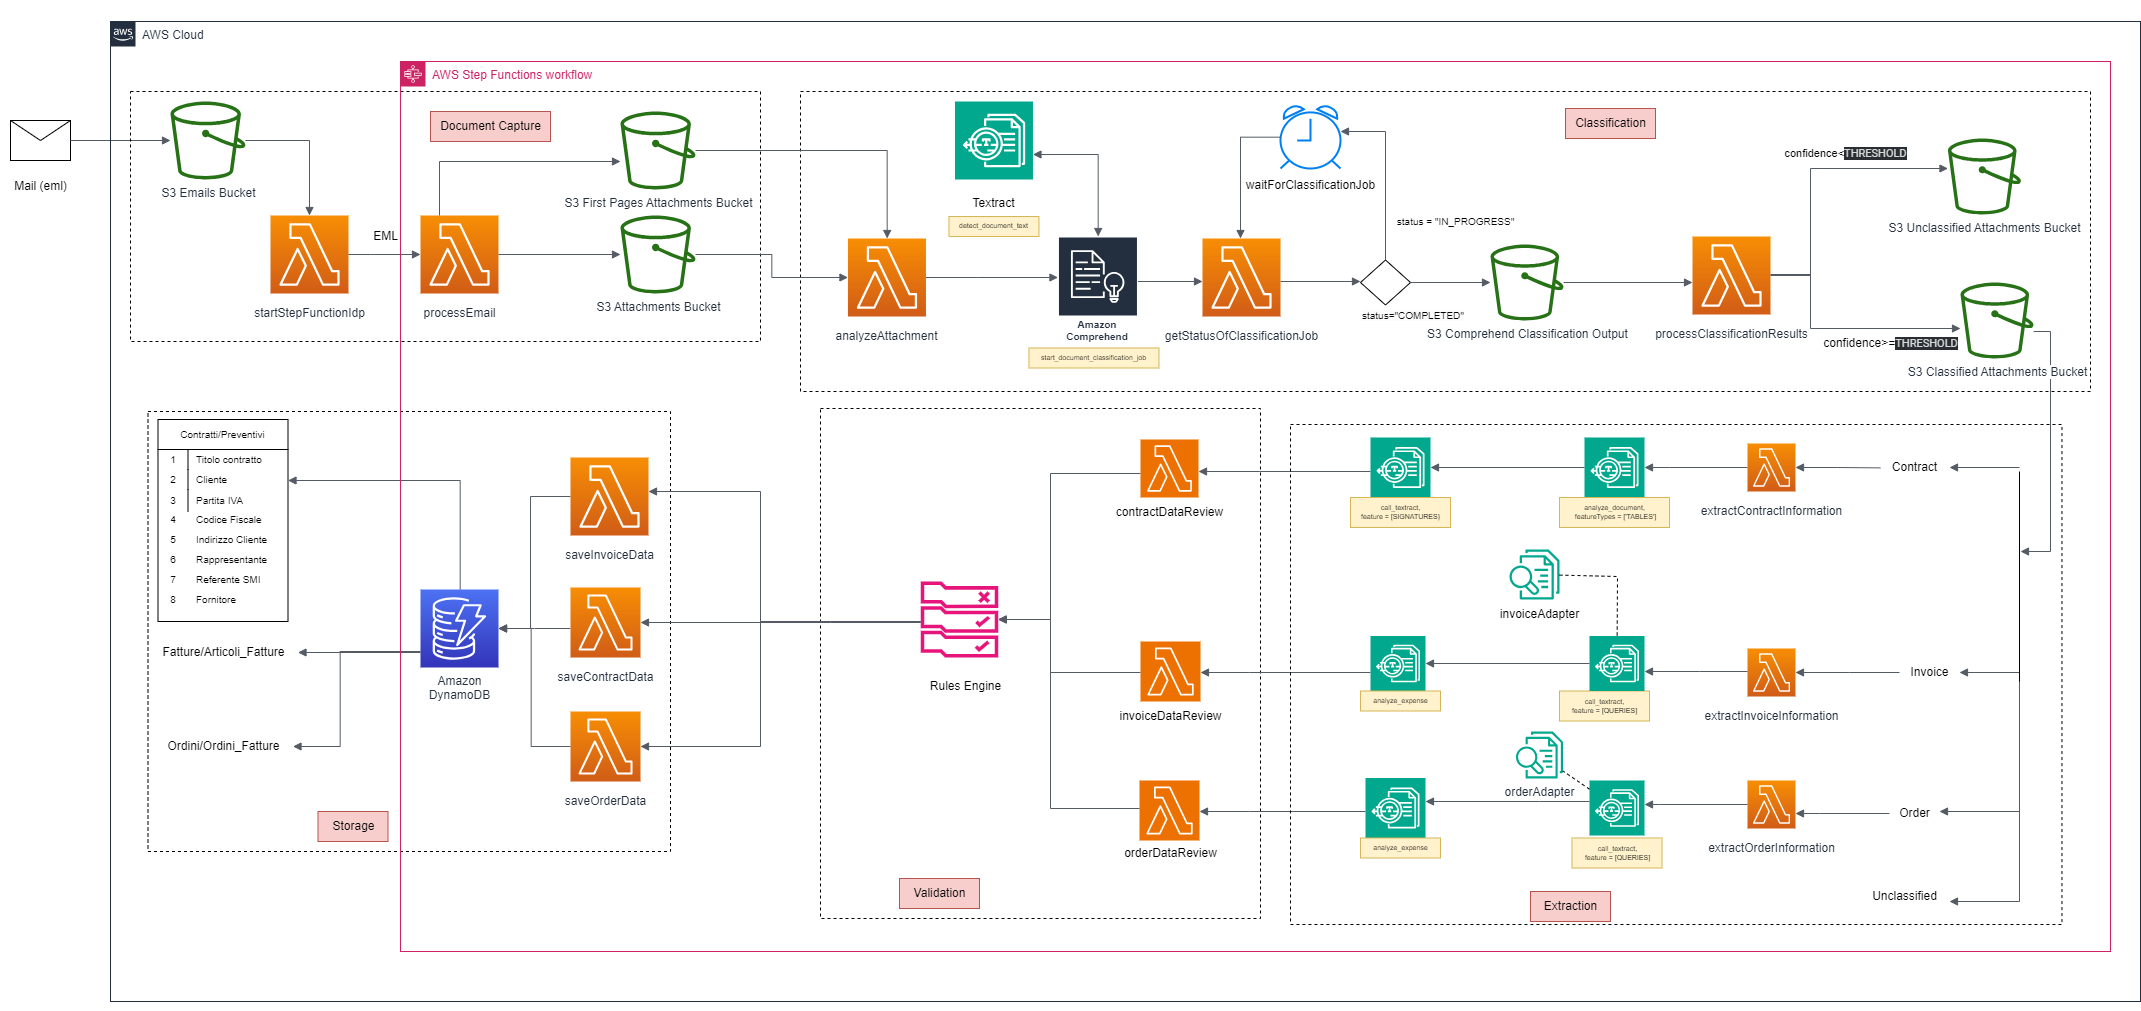
\includegraphics[width=\textheight]{img/design/classificatore_email.drawio.png}
    \end{turn}
    \captionof{figure}{Architettura ad alto livello del sistema}
    \label{fig:architettura-alto-livello}
\end{figure}

Come precedentemente menzionato, gran parte del flusso di lavoro è stato orchestrato tramite AWS Step Functions (nella figura \ref{fig:architettura-alto-livello} è evidenziato tramite un riquadro in rosso) e in particolare tramite la state machine denominata \emph{IdpStateMachine}. La figura \ref{fig:IDP_state_machine}, creata tramite l'editor di AWS, mostra la struttura della state machine e le diverse fasi coinvolte nel processo di elaborazione dei documenti.   
\begin{figure}[p]
    \centering
    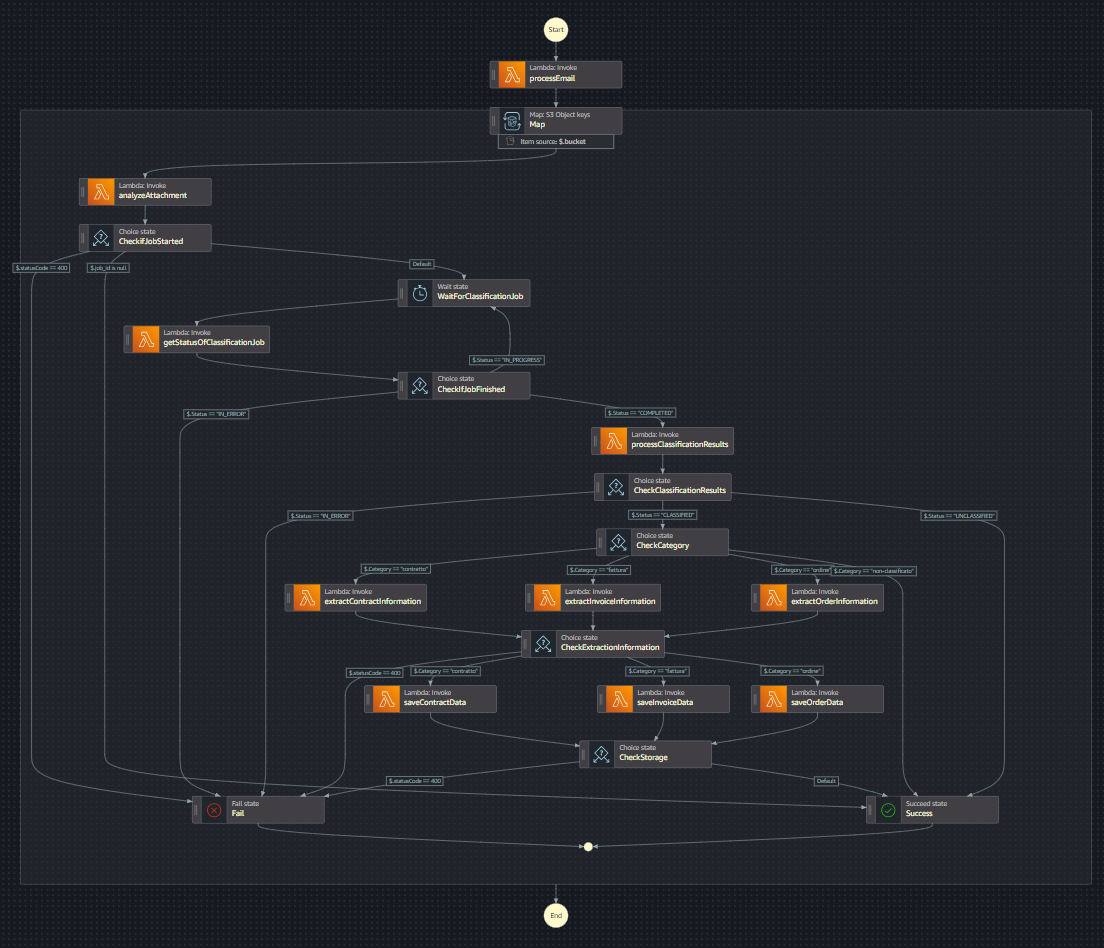
\includegraphics[width=1.1\textwidth, height=0.9\textheight]{img/design/IdpStateMachine.png}
    \caption{State machine "IdpStateMachine" di AWS Step Functions}
    \label{fig:IDP_state_machine}
\end{figure}
\section{Risorse e servizi AWS utilizzati}
\label{sec:risorse-servizi-aws}
Il sistema è stato progettato utilizzando una serie di risorse e servizi AWS, ciascuno dei quali svolge un ruolo specifico nel processo di elaborazione dei documenti. Le principali risorse e servizi utilizzati includono:
\begin{itemize}
    \item Amazon S3
    \begin{itemize}
        \item \emph{S3 Emails Bucket}: contenente le email in formato \texttt{.eml}.
        \item \emph{S3 Attachments Bucket}: contenente gli allegati estratti dalle email.
        \item \emph{S3 First Pages Attachments Bucket}: contenente le prime pagine dei file PDF estratte dagli allegati.
        \item \emph{S3 Comprehend Classification Output}: contenente i risultati della classificazione di Comprehend.
        \item \emph{S3 Classified Attachments Bucket}: contenente gli allegati classificati.
        \item \emph{S3 Unclassified Attachments Bucket}: contenente gli allegati non classificati.
    \end{itemize}
    \item AWS Lambda
    \begin{itemize}
        \item \emph{startStepFunctionIdp}: attiva l'esecuzione della state machine IdpStateMachine.
        \item \emph{processEmail}: estrae gli allegati dalle email.
        \item \emph{analyzeAttachment}: utilizza il classificatore di Comprehend per classificare gli allegati.
        \item \emph{getStatusOfClassificationJob}: controlla lo stato del job di classificazione.
        \item \emph{processClassificationResults}: elabora l'output della classificazione di Comprehend.
        \item \emph{extractContractInformation}: estrae le informazioni dai contratti.
        \item \emph{extractInvoiceInformation}: estrae le informazioni dalle fatture.
        \item \emph{extractOrderInformation}: estrae le informazioni dagli ordini.
        \item \emph{contractDataReview}: permette la revisione manuale delle informazioni estratte dai contratti.
        \item \emph{invoiceDataReview}: permette la revisione manuale delle informazioni estratte dalle fatture.
        \item \emph{orderDataReview}: permette la revisione manuale delle informazioni estratte dagli ordini.
        \item \emph{saveContractInformation}: salva le informazioni estratte dai contratti in DynamoDB.
        \item \emph{saveInvoiceInformation}: salva le informazioni estratte dalle fatture in DynamoDB.
        \item \emph{saveOrderInformation}: salva le informazioni estratte dagli ordini in DynamoDB.
    \end{itemize}
    \item AWS Step Functions
    \begin{itemize}
        \item \emph{IdpStateMachine}: gestisce il flusso di lavoro.
    \end{itemize}
    \item Amazon Comprehend
    \begin{itemize}
        \item \emph{document-classifier}: modello personalizzato per la classificazione degli allegati.
        \item \emph{custom-document-classifier-flywheel}: flywheel per la creazione di modelli personalizzati che riporta tre differenti \gls{datasetg}:
        \begin{itemize}
            \item \emph{document-classifier-train}: \gls{datasetg} di training per la prima versione del modello.
            \item \emph{trainingFatture}: \gls{datasetg} di training per la seconda versione del modello.
            \item \emph{my-training-set}: \gls{datasetg} di training per la seconda versione del modello.
        \end{itemize}
    \end{itemize}
    \item Amazon Textract
    \begin{itemize}
        \item \emph{analyze\_document}: estrae le informazioni principali dai documenti.
        \item \emph{call\_textract}: funzione simile a \emph{analyze\_document} ma con funzionalità aggiuntive.
        \item \emph{adapter checksInvoiceAdapter}: adattatore utilizzato per le custom queries per l'estrazione delle informazioni dalle fatture.
        \item \emph{adapter checksOrderAdapter}: adattatore utilizzato per le custom queries per l'estrazione delle informazioni dagli ordini.
    \end{itemize}
    \item Amazon DynamoDB
    \begin{itemize}
        \item \emph{Contratti}: tabella contenente le informazioni estratte dai contratti.
        \item \emph{Preventivi}: tabella contenente le informazioni estratte dai preventivi.
        \item \emph{Fatture}: tabella contenente le informazioni estratte dalle fatture.
        \item \emph{Articoli\_Fatture}: tabella contenente le informazioni relative agli articoli delle fatture.
        \item \emph{Ordini}: tabella contenente le informazioni estratte dagli ordini.
        \item \emph{Articoli\_Ordini}: tabella contenente le informazioni relative agli articoli degli ordini.
    \end{itemize}
\end{itemize}
\section{Estrazione degli allegati}
\label{sec:estrazione-allegati}
Inizialmente, l'indicazione fornita dall'azienda richiedeva un'analisi del contenuto delle email, seguita da una classificazione basata sull'elaborazione del linguaggio naturale e sui metadati contenuti. Tuttavia, con il chiarimento delle categorie di interesse (ordini, fatture e contratti), ho deciso di concentrare l'attenzione sull'estrazione degli allegati presenti nelle email piuttosto che sul contenuto testuale delle stesse.

Questa scelta è giustificata dal fatto che i documenti di interesse per l'azienda sono spesso inclusi come allegati nelle email, rendendo l'estrazione degli allegati un approccio più diretto ed efficace. Inoltre, il contenuto delle email è spesso irrilevante o solo parzialmente utile per il processo di classificazione.

L'obiettivo principale di questa fase è quindi quello di ricavare gli allegati dalle email per poterli successivamente classificare e analizzare. Il processo è strutturato nelle seguenti fasi:

\begin{itemize}
    \item \textbf{Caricamento del file \texttt{.eml}}: Il processo inizia con il caricamento del file \texttt{.eml} nel bucket "S3 Emails Bucket", che funge da archivio per le email da analizzare.
    
    \item \textbf{Attivazione della funzione Lambda "StartStepFunctionIdp"}: L'inserimento del file \texttt{.eml} nel bucket attiva la funzione Lambda \emph{StartStepFunctionIdp}, la quale avvia l'esecuzione della state machine \emph{IdpStateMachine} di AWS \emph{Step Functions}. Questa state machine gestisce l'intero flusso di lavoro automatizzato.

    \item \textbf{Estrazione degli allegati}: La state machine avvia la funzione Lambda \emph{processEmail}, responsabile dell'estrazione degli allegati dalle email. Questa funzione è essenziale per isolare i documenti di interesse dal file \texttt{.eml}.
    \item \textbf{Caricamento degli allegati}: Una volta estratti, gli allegati vengono caricati nel bucket \emph{S3 Attachments Bucket}. Gli allegati, che possono essere in vari formati (PDF, PNG, JPG, TXT, DOC, DOCX, ecc.), vengono archiviati in una cartella il cui nome corrisponde a quello della mail da cui provengono (file \texttt{.eml}). In aggiunta, le prime pagine dei file PDF vengono salvate nel bucket \emph{S3 First Pages Attachments Bucket} e vengono archiviati nello stesso modo. 
\end{itemize}
Gli allegati, ora presenti nei bucket \emph{S3 Attachments Bucket} e \emph{S3 First Pages Attachments Bucket}, sono pronti per essere classificati e analizzati nelle fasi successive del processo. 
\section{Classificazione dei documenti}
\label{sec:classificazione-documenti}
Inizialmente, si era presa in considerazione l'idea di classificare le email in base al loro contenuto utilizzando modelli di \gls{mlg} offerti da \emph{Amazon SageMaker}. Tuttavia, con il chiarimento delle categorie di interesse durante lo stage (ordini, fatture e contratti), si è deciso di focalizzarsi sull'estrazione e la classificazione degli allegati presenti nelle email, piuttosto che sul contenuto testuale delle stesse. Questo approccio ha semplificato significativamente il processo di classificazione, poiché i metadati (denominati anche \textit{features} nel contesto del \gls{mlg}) si riducono al semplice testo estratto dagli allegati e tale caso d'uso si presta bene all'utilizzo di \emph{Amazon Comprehend} per la classificazione ed in particolare per la creazione di un modello personalizzato.\\
Sebbene in una fase iniziale fosse stato considerato e provato l'uso del servizio \emph{Amazon Bedrock} per classificare i documenti, in particolare con il modello \emph{Claude-3}, questa opzione è stata successivamente scartata a favore di un modello personalizzato, ritenuto più adatto alle specifiche esigenze del progetto e meno costoso.\\
In questo contesto, l'utilizzo di \emph{Amazon Textract} e \emph{Amazon Comprehend} si è rivelato cruciale per l'accuratezza della classificazione.\\
La fase di classificazione degli allegati (figura \ref{fig:architettura-alto-livello} riquadro denominato \emph{Classification}) si articola nelle seguenti operazioni:

\begin{itemize}
    \item \textbf{Caricamento del file \texttt{.eml} e attivazione della pipeline}: Dopo l'estrazione degli allegati dalle email, descritta nella Sezione \ref{sec:estrazione-allegati}, i documenti vengono preparati per la classificazione. La funzione Lambda \emph{analyzeAttachment} utilizza il classificatore di Amazon Comprehend denominato 
    \emph{document-classifier} per analizzare la prima pagina degli allegati ricavandole dal bucket \emph{S3 First Pages Attachments Bucket}. Il testo viene estratto tramite la funzione \texttt{detect\_document\_text} di \emph{Amazon Textract}, che converte i contenuti dei documenti in un formato testuale adatto per l'analisi.

    \item \textbf{Salvataggio del risultato della classificazione}: I risultati del job di classificazione, composti da un file JSON che riporta la categoria assegnata e il relativo livello di confidenza, vengono salvati nel bucket \emph{S3 Comprehend Classification Output}. Questo passaggio consente di archiviare in modo strutturato i risultati che saranno successivamente elaborati per l'estrazione delle informazioni.

    \item \textbf{Processamento dei risultati della classificazione}: Al termine del job di classificazione, la funzione Lambda \emph{processClassificationResults} viene attivata per salvare gli allegati classificati nei \emph{bucket} appropriati. Infatti se la confidenza del modello è superiore a una soglia (\textit{threshold}) predefinita, l'allegato viene salvato nel \emph{bucket} \emph{S3 Classified Attachments Bucket}; altrimenti, viene salvato nel \emph{bucket} \emph{S3 Unclassified Attachments Bucket}. Gli allegati sono archiviati in cartelle che riportano la categoria di classificazione (ordine, fattura, contratto, non classificato). Questa organizzazione è fondamentale per facilitare la gestione e l'analisi successiva degli allegati, compresi quelli non classificati, che possono essere esaminati in dettaglio in un secondo momento.
\end{itemize}

Una precisazione importante riguarda la distinzione tra gli allegati salvati nel bucket \emph{S3 Classified Attachments Bucket} e quelli salvati nel bucket \emph{S3 Unclassified Attachments Bucket} 
all'interno della cartella "non classificato". Gli allegati presenti nel bucket \emph{S3 Unclassified Attachments Bucket} sono quelli per cui il livello di confidenza del modello è inferiore alla soglia predefinita. Al contrario, gli allegati presenti nella cartella "non classificato" del \emph{S3 Classified Attachments Bucket} sono stati classificati con una confidenza superiore alla soglia, ma la categoria assegnata è comunque "non classificato", indicando la classificazione sia stata effettuata con un certo grado di sicurezza.
\subsection{Creazione del modello di classificazione personalizzato}
\label{subsec:training-modello}
La creazione di un modello di classificazione personalizzato con Amazon Comprehend richiede la disponibilità di un \gls{datasetg} ampio, significativo e bilanciato, capace di distinguere con precisione le categorie di interesse. È fondamentale che il \gls{datasetg} sia etichettato correttamente, in modo che ogni documento sia associato alla giusta categoria di appartenenza.

Durante la fase di etichettatura, sono emerse alcune considerazioni chiave. I documenti da analizzare sono prevalentemente file PDF, spesso costituiti da scansioni. Per garantire coerenza nel processo di training, si è deciso di utilizzare esclusivamente documenti in formato PDF. Inoltre, è stato scelto di utilizzare unicamente le prime pagine di tali documenti per il training del modello. Questa scelta è stata motivata dal fatto che le prime pagine contengono generalmente le informazioni più rilevanti per la classificazione. Inoltre, considerando che il costo dell'analisi è proporzionale al numero di pagine, la riduzione del numero di pagine ha comportato una significativa riduzione dei costi operativi, soprattutto in documenti che possono arrivare fino a 30 o più pagine.

Tuttavia, queste scelte hanno anche portato a una riduzione della varietà dei dati utilizzati per il training, il che potrebbe potenzialmente introdurre \glsfirstoccur{\gls{biasg}} nel modello, limitando la sua capacità di generalizzare su nuovi dati. \\
Del modello personalizzato denominato \emph{document-classifier} sono state create due versioni, ciascuna addestrata su dei \gls{datasetg} specifici. 
Per la prima versione del modello, denominata \emph{document-classifier-version-1}, sono stati utilizzati 47 documenti etichettati.\\
Per la seconda versione del modello, denominata \emph{Comprehend-Generated-v1-
461f932}, generata tramite il processo di \gls{activelearningg} con \emph{Flywheel}, sono stati utilizzati dei \gls{datasetg} di training di 56 documenti che si vanno ad aggiungere ai 47 documenti utilizzati per la versione precedente.
Per creare e distribuire il modello personalizzato, sono state seguite le seguenti fasi: \emph{Analisi del dataset}, \emph{Preprocessing}, \emph{Training}, \emph{Valutazione} e \emph{Test del modello}.
\paragraph*{Analisi del dataset}
L'\emph{analisi del dataset} è fondamentale per comprendere la distribuzione delle categorie e valutare l'adeguatezza dei dati per la successiva fase di addestramento. Per i \gls{datasetg} utilizzati nelle varie iterazioni, le percentuali di distribuzione delle categorie (ordini, fatture, contratti e non classificato) sono state attentamente monitorate per garantire un bilanciamento adeguato.\\
Per il primo dataset di training, denominato \emph{document-classifier-train}, sono stati utilizzati 47 documenti etichettati, distribuiti nel modo seguente:
\begin{itemize}
    \item 25 contratti (53.19\%)
    \item 3 fatture (6.38\%)
    \item 5 ordini (10.64\%)
    \item 14 non classificati (29.79\%)
\end{itemize}
Per il secondo dataset di training, denominato \emph{trainingFatture}, sono stati utilizzati 26 documenti etichettati, distribuiti nel modo seguente:
\begin{itemize}
    \item 1 ordine (3.85\%)
    \item 25 fatture (96.15\%)
\end{itemize}
Per il terzo dataset di training, denominato \emph{my-training-set}, sono stati utilizzati 30 documenti etichettati, distribuiti nel modo seguente:
\begin{itemize}
    \item 10 fatture (33.33\%)
    \item 10 non classificati (33.33\%)
    \item 10 ordini (33.33\%)
\end{itemize}
Tali scelte sono state guidate dalla necessità di garantire un bilanciamento adeguato delle categorie, in modo da evitare che il modello sia influenzato da una distribuzione sbilanciata dei dati. Inoltre, è stato fondamentale assicurare che i documenti etichettati fossero rappresentativi delle categorie di interesse, in modo da garantire che il modello fosse in grado di generalizzare su nuovi dati.

\paragraph*{Preprocessing}
Il preprocessing dei dati è una fase critica del processo di addestramento. Le operazioni principali sono state:

\begin{itemize}
    \item \textbf{Estrazione del testo tramite Amazon Textract}: Il testo contenuto nelle prime pagine dei PDF è stato estratto utilizzando \emph{Amazon Textract} tramite l'\gls{apig} \texttt{call\_textract}. 
    \item \textbf{Creazione del file CSV}: I dati estratti sono stati organizzati in un file CSV, con una colonna per la categoria di classificazione e una per il testo.
    \item \textbf{Caricamento del file CSV}: Il file di training CSV è stato caricato su \emph{Amazon S3} tramite \emph{Flywheel}, per essere utilizzato nel processo di \emph{training}.
\end{itemize}

\paragraph*{Training}
Durante la fase di {training}, il file CSV creato in precedenza è stato utilizzato per addestrare una nuova versione del classificatore personalizzato all'interno di \emph{Amazon Comprehend}. Il processo di training è stato eseguito utilizzando il servizio \emph{Flywheel}, che consente di creare e gestire modelli personalizzati in modo efficiente. Il modello è stato addestrato su un'istanza \emph{ml.m5.xlarge} per garantire prestazioni ottimali e tempi di risposta rapidi.

\paragraph*{Valutazione}
La valutazione del modello è stata condotta utilizzando metriche standard, che hanno riportato i seguenti risultati per entrambe le versioni del modello:
\begin{itemize}
    \item Precision: 1.0
    \item Recall: 1.0
    \item F1: 1.0
    \item Accuracy: 1.0
    \item Micro precision: 1.0
    \item Micro recall: 1.0
    \item Micro F1: 1.0
\end{itemize}
Questi risultati indicano una performance ottimale del modello sulle classi di interesse.\\
TO DO: spiegare meglio le metriche di valutazione.

\paragraph*{Test del modello}
Per testare il modello, è sufficiente caricare il file desiderato in un \emph{bucket S3} e avviare un \emph{job} di classificazione. Il modello restituirà la categoria di classificazione assegnata al documento e il livello di confidenza associato, permettendo così una verifica immediata delle sue prestazioni.

\subsection{Processo di Active Learning con Flywheel}
Per migliorare il modello nel tempo, è stato utilizzato il processo di \glsfirstoccur{\gls{activelearningg}} implementato tramite il servizio \emph{Flywheel} di \emph{Amazon Comprehend}. Questo approccio consente di iterare sul modello, migliorandolo progressivamente sulla base dei nuovi dati e delle prestazioni ottenute. Il processo segue questi passaggi:

\begin{itemize}
    \item \textbf{Creazione di un \emph{dataset Flywheel}}: Si parte con la definizione di un \emph{dataset} contenente i documenti etichettati, che verrà utilizzato per l'addestramento del modello.
    \item \textbf{Inizializzazione di un'iterazione \emph{Flywheel}}: Viene avviata un'iterazione di \emph{Flywheel}, durante la quale il modello viene addestrato sui dati disponibili.
    \item Attivazione del nuovo modello: Sulla base dei risultati dell'iterazione, viene deciso se attivare il nuovo modello. La decisione si basa su parametri predefiniti, come le metriche di precisione, recall e F1 score.
\end{itemize}

\section{Estrazione delle informazioni}
In questa fase l'obiettivo è l'estrazione delle informazioni associate a ciascuna categoria escludendo la categoria non classificato. A partire dai risultati di classificazione della fase precedente si è analizzato il metodo migliore per poter estrarre le informazioni ricercate dalle categorie di contratti, ordini e fatture. Per ciascuna categoria
utilizzata una funzione \emph{lambda} che tramite \emph{Amazon Textract} estrae le informazioni
principali dai documenti. Per ciascuna delle informazioni estratte viene riportata
anche la confidenza associata utile nella fase successiva.\\
Fondamentalmente sono stati analizzati diversi metodi utilizzando differenti servizi per aderire a tale scopo:
\begin{itemize}
    \item Comprehend custom entities
    \item Amazon Bedrock con il modello Claude-3
    \item Servizi di Amazon Textract
\end{itemize}
Per ciascuna categoria è stata fatta dunque un'analisi che ha riguardato i costi oltre che l'efficacia del servizio.\\
\subsection{Estrazione delle informazioni dai contratti}
\label{subsec:estrazione-contratti}
Per l'estrazione delle informazioni dai contratti, è stata adottata una soluzione efficace e a basso costo, sfruttando la struttura uniforme di questi documenti. I contratti analizzati presentano una tabella standardizzata che contiene le seguenti informazioni chiave:

\begin{itemize}
    \item Titolo del contratto
    \item Cliente
    \item Partita IVA del cliente
    \item Codice fiscale del cliente
    \item Indirizzo del cliente
    \item Rappresentante legale del cliente
    \item Referente SMI
    \item Fornitore
\end{itemize}

La strategia implementata si basa sull'identificazione di questa tabella e sull'estrazione automatizzata dei campi utilizzando le conoscenze predefinite sulla struttura del documento. Per estrarre le informazioni desiderate, è stato impiegato \emph{Amazon Textract}, utilizzando la funzione \texttt{analyze\_document} con l'opzione \texttt{TABLES}, che consente di estrarre in modo efficiente i dati tabulari presenti nella prima pagina del contratto.

Per distinguere tra preventivi e contratti, è stata adottata una strategia basata sulla rilevazione delle firme all'interno del documento, sempre utilizzando \emph{Amazon Textract}, ma con la funzione \texttt{SIGNATURES}. Il processo prevede l'analisi delle pagine a partire dall'ultima, alla ricerca di firme. Se una firma viene rilevata, il documento viene classificato come contratto. Se, invece, al termine dell'analisi di tutte le pagine, non viene trovata alcuna firma, il documento viene classificato come preventivo.

Il risultato di questa analisi viene salvato in un file JSON di output, includendo un campo \texttt{is\_contract} che indica se il documento è stato classificato come contratto o preventivo. In caso di rilevamento di una firma, viene registrato anche il livello di confidenza associato. Se non viene trovata alcuna firma, la classificazione come preventivo viene effettuata con una confidenza del 100\%. In entrambi i casi, viene applicata una soglia (\textit{threshold}) di confidenza per garantire l'accuratezza del processo di rilevazione delle firme.

Questa soluzione permette di distinguere in modo efficace tra contratti e preventivi, sfruttando le funzionalità avanzate di \emph{Amazon Textract} e mantenendo i costi operativi contenuti, senza compromettere l'affidabilità e la precisione del processo.

\subsection{Estrazione delle informazioni dalle fatture}
\label{subsec:estrazione-fatture}
Per l'estrazione delle informazioni dalle fatture, sono state considerate diverse tecnologie, valutandone costi ed efficacia. Le soluzioni analizzate includono:

\begin{itemize}
    \item Amazon Textract, in particolare la funzione \texttt{analyze\_expense}
    \item Comprehend Custom Entity Recognition
    \item Amazon Bedrock con il modello Claude-3
    \item Utilizzo di \textit{queries} e \textit{custom queries} (adapters) di Amazon Textract
\end{itemize}

Per quanto riguarda l'analisi delle fatture tramite la funzione \texttt{analyze\_expense} di Amazon Textract, questa è stata presa in considerazione poiché è specificamente progettata per l'analisi di fatture e ricevute, offrendo un'alta precisione per layout standard. Tuttavia, la sua efficacia è limitata a questi layout predefiniti e potrebbe non essere ottimale per fatture con strutture non convenzionali.

L'utilizzo di Comprehend Custom Entity Recognition consente di creare un modello personalizzato per l'estrazione di entità specifiche dalle fatture. Offre un'elevata precisione e flessibilità nell'adattarsi a layout variabili, ma presenta costi elevati e richiede un significativo sforzo nella preparazione e annotazione dei dati di addestramento.

Amazon Bedrock con il modello Claude-3 è stato valutato per la sua capacità di gestire layout complessi e variabili, garantendo un'elevata precisione. Tuttavia, il modello non è specificamente addestrato sui dati aziendali, il che potrebbe ridurre la sua efficacia per esigenze particolari.

L'utilizzo di \textit{queries} e \textit{custom queries} tramite \textit{adapters} di Amazon Textract è stato infine scelto per l'analisi delle fatture grazie alla sua elevata precisione e flessibilità nel gestire layout variabili. Questa soluzione offre un buon compromesso tra personalizzazione, costi e precisione, con tempi di addestramento del modello inferiori rispetto ad altri metodi.

La soluzione basata su \textit{queries} è risultata la più conveniente, offrendo un valore elevato di precisione per un numero limitato di fatture. L'integrazione con gli \textit{adapters}, in particolare l'uso dell'\textit{adapter} "checksInvoiceAdapter", ha garantito una personalizzazione ottimale mantenendo i costi contenuti.

Le informazioni principali estratte dalle fatture con questa soluzione sono:

\begin{itemize}
    \item Numero fattura
    \item Data fattura
    \item Venditore
    \item Prezzo totale
    \item Partita IVA del venditore
    \item Codice fiscale del venditore
    \item Imponibile
    \item Imposta
\end{itemize}

Per quanto riguarda l'estrazione delle informazioni relative agli articoli delle fatture, l'utilizzo della funzione \texttt{analyze\_expense} di Amazon Textract è emerso come la soluzione più efficace. Questa tecnologia offre un'elevata precisione e flessibilità nel gestire layout variabili, risultando particolarmente adatta per l'estrazione delle seguenti informazioni:

\begin{itemize}
    \item Codice articolo
    \item Descrizione articolo
    \item Valore unitario
    \item Quantità
    \item Unità di misura
    \item Sconto percentuale
    \item IVA
    \item Imponibile articolo
\end{itemize}

Questa combinazione di strumenti e tecnologie ha permesso di ottimizzare il processo di estrazione delle informazioni dalle fatture, garantendo un'elevata accuratezza e adattabilità a diverse tipologie di documenti.


\subsection{Estrazione delle informazioni dagli ordini}
In questa fase si possono applicare considerazioni simili a quelle discusse per l'estrazione delle informazioni dalle fatture (sezione \ref{subsec:estrazione-fatture}), poiché sono state prese in considerazione le stesse tecnologie, con problematiche analoghe.

Per l'estrazione delle informazioni principali dagli ordini, i campi identificati sono i seguenti:

\begin{itemize}
    \item Numero ordine
    \item Data ordine
    \item Venditore
    \item Prezzo totale
    \item Partita IVA del venditore
    \item Codice fiscale del venditore
    \item Imponibile
    \item Imposta
\end{itemize}

Queste informazioni vengono estratte dai documenti utilizzando le \textit{queries} di Amazon Textract, integrate con \textit{custom queries} (\textit{adapters}) per adattarsi a layout variabili. L'\textit{adapter} utilizzato in questo contesto è denominato "checksOrderAdapter".

Per quanto riguarda l'estrazione delle informazioni relative agli articoli contenuti negli ordini, l'utilizzo della funzione \texttt{analyze\_expense} di Amazon Textract è emerso come la soluzione più efficace. Questa tecnologia offre un'elevata precisione e flessibilità, adattandosi a diversi layout. Le informazioni estratte per ciascun articolo sono le seguenti:

\begin{itemize}
    \item Codice articolo
    \item Descrizione articolo
    \item Valore unitario
    \item Quantità
    \item Unità di misura
    \item Sconto percentuale
    \item IVA
    \item Imponibile articolo
    \item Data consegna
\end{itemize}

L'adozione di queste tecnologie ha permesso di ottimizzare il processo di estrazione delle informazioni dagli ordini, garantendo un'elevata accuratezza e adattabilità a diverse tipologie di documenti, analogamente a quanto avviene per le fatture.

\subsection{Creazione degli adapter}
Gli \textit{adapter} sono stati creati per personalizzare le query di Amazon Textract, consentendo l'estrazione di informazioni specifiche dai documenti. Questi \textit{adapter} sono stati utilizzati per l'estrazione delle informazioni sia dalle fatture che dagli ordini, e sono denominati rispettivamente \textit{checksInvoiceAdapter} e \textit{checksOrderAdapter}.

\subsubsection{ChecksInvoiceAdapter}
L'\textit{adapter} \textit{checksInvoiceAdapter} è stato sviluppato per l'estrazione delle informazioni dalle fatture. Le query personalizzate configurate in questo \textit{adapter} sono state pensate per coprire tutte le informazioni rilevanti, tra cui date, importi, identificativi e dettagli degli articoli. Le query utilizzate includono:

\begin{itemize}
    \item What is the invoice date or billing date?
    \item What is the invoice ID or billing number?
    \item What is the total tax amount?
    \item What is the receiver tax ID?
    \item What is the bill to name?
    \item What is the vendor name?
    \item What is the vendor VAT number?
    \item What is the vendor taxpayer ID?
    \item What is the subtotal?
    \item What is the tax?
    \item What is the total?
    \item What are the article codes? (Articolo in Italian)
    \item What are the descriptions of the items?
    \item What are the unit prices of the articles? (Valore in Italian)
    \item What are the quantities per item?
    \item What are the units of measure for the items?
    \item What are the discounts per item?
    \item What is the VAT rate per item? (IVA in Italian)
    \item What are the taxable amounts per article? (Imponibile in Italian)
    \item How many items are listed in this invoice?
\end{itemize}

L'\textit{adapter}, attualmente alla sesta versione, è stato addestrato su un dataset di 21 fatture, di cui 16 utilizzate per il training e 5 per il test.

\subsubsection{ChecksOrderAdapter}
L'\textit{adapter} \textit{checksOrderAdapter} è stato creato per l'estrazione delle informazioni dagli ordini. Anche in questo caso, le query sono state personalizzate per garantire un'accurata estrazione dei dati rilevanti, come le date, gli importi e i dettagli degli articoli. Le query configurate includono:

\begin{itemize}
    \item What is the order date?
    \item What is the order ID?
    \item What is the bill to name?
    \item What is the internal code of the order?
    \item What is the taxpayer ID?
    \item What is the item amount in this order?
    \item What is the net amount in this order?
    \item What is the total amount in this order?
    \item What are the article codes? (Articolo in Italian)
    \item What are the descriptions of the items?
    \item What are the quantities per item?
    \item What are the units of measure for the items?
    \item What are the discounts per item?
    \item What are the delivery dates for each item?
\end{itemize}

L'\textit{adapter}, attualmente alla seconda versione, è stato addestrato su un dataset di 10 ordini, di cui 5 utilizzati per il training e 5 per il test.

Questi \textit{adapter} hanno permesso di migliorare significativamente la precisione e l'efficacia dell'estrazione delle informazioni dalle fatture e dagli ordini, adattandosi ai layout variabili dei documenti e garantendo un'alta qualità dei dati estratti.
\section{Validazione delle informazioni}
In questa fase, le informazioni estratte dai documenti vengono sottoposte a un processo di validazione. Per ciascuna categoria di documento (ordine, fattura, contratto) è stata implementata una funzione Lambda specifica per la validazione dei dati. La strategia di validazione applicata varia in base alla categoria di appartenenza, con regole specifiche per ogni tipo di dato. Se una delle regole di validazione non viene rispettata, il dato viene considerato non valido.

\subsection{Validazione dei contratti}
\label{subsec:validazione-contratti}
Per i contratti, le seguenti regole di validazione sono state definite:

\begin{itemize}
    \item \textbf{Titolo contratto}: obbligatorio
    \item \textbf{Cliente}: obbligatorio
    \item \textbf{is\_contract}: obbligatorio e di tipo booleano
    \item \textbf{Partita IVA del cliente}: obbligatoria
\end{itemize}

Sono inoltre state stabilite soglie di confidenza per ciascuna delle informazioni estratte. Se la confidenza è inferiore alla soglia stabilita, il dato viene considerato non valido. Ad eccezione del "Titolo contratto" (per cui la soglia è 0.8), la soglia scelta per le altre informazioni è pari a 0.9.

\subsection{Validazione delle fatture}
\label{subsec:validazione-fatture}
Per le informazioni generali delle fatture, sono state definite le seguenti regole di validazione:

\begin{itemize}
    \item \textbf{Numero fattura}: obbligatorio
    \item \textbf{Data fattura}: deve avere un formato valido
    \item \textbf{Imposta}: deve essere un numero
    \item \textbf{Imponibile}: deve essere un numero
    \item \textbf{Prezzo totale}: deve essere un numero
    \item \textbf{Partita IVA}: deve avere una lunghezza di 11 caratteri e deve essere un numero
\end{itemize}

Per le informazioni relative agli articoli delle fatture, sono state definite le seguenti regole di validazione:

\begin{itemize}
    \item \textbf{Valore unitario}: deve essere un numero
    \item \textbf{Quantità}: deve essere un numero
    \item \textbf{IVA}: deve essere un numero
    \item \textbf{Imponibile articolo}: deve essere un numero
\end{itemize}

\subsection{Validazione degli ordini}
\label{subsec:validazione-ordini}
Per le informazioni generali degli ordini, le regole di validazione stabilite sono le seguenti:

\begin{itemize}
    \item \textbf{Codice interno}: obbligatorio
    \item \textbf{Data ordine}: deve avere un formato valido
    \item \textbf{Prezzo totale}: deve essere un numero
    \item \textbf{Partita IVA}: deve avere una lunghezza di 11 caratteri
\end{itemize}

Per le informazioni relative agli articoli degli ordini, sono state stabilite le seguenti regole di validazione:

\begin{itemize}
    \item \textbf{Valore unitario}: deve essere un numero
    \item \textbf{Quantità}: deve essere un numero
    \item \textbf{IVA}: deve essere un numero
    \item \textbf{Imponibile articolo}: deve essere un numero
    \item \textbf{Data consegna}: deve avere un formato valido
\end{itemize}

In tutte le categorie, la validazione delle informazioni è cruciale per garantire l'integrità e l'accuratezza dei dati processati. Le soglie di confidenza e le regole definite permettono di filtrare i dati non validi, migliorando l'affidabilità del sistema.

\section{Persistenza dei dati}
L'obiettivo di questa fase è garantire la persistenza dei dati estratti. La scelta per la memorizzazione dei risultati è ricaduta su Amazon DynamoDB, grazie alla sua scalabilità e affidabilità. Il flusso di lavoro prevede l'utilizzo di funzioni Lambda dedicate per ciascuna categoria di documenti (contratti, ordini, fatture), che si occupano di salvare i dati estratti nelle rispettive tabelle di DynamoDB.
Per ciascuna categoria di documenti è stata creata una funzione Lambda specifica, che salva i risultati nelle seguenti tabelle di DynamoDB:
\begin{itemize}
    \item \textbf{Contratti}: Salva i dati relativi ai contratti nella tabella \texttt{Contratti} o, in caso di documenti classificati come preventivi, nella tabella \texttt{Preventivi}. La distinzione viene effettuata sulla base della variabile \texttt{is\_contract} presente nel file JSON di output.
    \item \textbf{Fatture}: Salva le informazioni generali delle fatture nella tabella \texttt{Fatture} e gli articoli associati nella tabella \texttt{Articoli\_Fatture}.
    \item \textbf{Ordini}: Salva le informazioni generali degli ordini nella tabella \texttt{Ordini} e gli articoli associati nella tabella \texttt{Articoli\_Ordini}.
\end{itemize}

\subsection{Contratti}
Le informazioni estratte dai contratti vengono salvate nella tabella \texttt{Contratti} di DynamoDB. Se il documento viene identificato come preventivo, i dati vengono invece memorizzati nella tabella \texttt{Preventivi}. Questa distinzione si basa sul valore della variabile \texttt{is\_contract} ottenuta durante l'analisi.

\subsection{Fatture}
Le informazioni generali delle fatture vengono salvate nella tabella \texttt{Fatture} di DynamoDB. Inoltre, ogni articolo associato alla fattura viene memorizzato separatamente nella tabella \texttt{Articoli\_Fatture}, assicurando una gestione dettagliata e strutturata delle informazioni.

\subsection{Ordini}
Le informazioni generali degli ordini vengono salvate nella tabella \texttt{Ordini} di DynamoDB. Similmente alle fatture, gli articoli associati agli ordini vengono memorizzati nella tabella \texttt{Articoli\_Ordini}, permettendo di gestire in modo efficace i dettagli relativi a ciascun ordine.

Questo approccio assicura che tutti i dati estratti dai documenti siano memorizzati in modo organizzato e facilmente accessibile, sfruttando le potenzialità di DynamoDB per garantire performance elevate e affidabilità nel tempo.

\section{Analisi dei costi}
TO DO
%\section{Tecnologie e strumenti}
%\label{sec:tecnologie-strumenti}
%
%Di seguito viene data una panoramica delle tecnologie e strumenti utilizzati.
%
%\subsection*{Tecnologia 1}
%Descrizione Tecnologia 1.
%
%\subsection*{Tecnologia 2}
%Descrizione Tecnologia 2
%
%\section{Ciclo di vita del software}
%\label{sec:ciclo-vita-software}
%
%\section{Progettazione}
%\label{sec:progettazione}
%
%\subsection{Namespace 1} %**************************
%Descrizione namespace 1.
%
%\begin{namespacedesc}
%    \classdesc{Classe 1}{Descrizione classe 1}
%    \classdesc{Classe 2}{Descrizione classe 2}
%\end{namespacedesc}
%
%
%\section{Design Pattern utilizzati}
%
%\section{Codifica}


    \chapter{Sviluppi futuri}
\label{cap:sviluppi-futuri}
\emph{In questa sezione vengono proposti alcuni sviluppi futuri del sistema.}
\section{Analisi del contenuto della mail}
Per poter analizzare il contenuto della mail ed estrarre le informazioni associate si può modificare la funzione lambda \textit{processEmail} in modo tale da estrarre il testo della mail e non solo gli allegati ed eventualmente caricarlo su un altro bucket S3.\\
Inoltre, si può implementare un modello di classificazione di Comprehend per classificare il testo della mail in base al contenuto analogamente a quanto fatto per gli allegati e successivamente estrarre le informazioni associate. 
\section{Aggiunta di nuove categorie}
Si possono aggiungere nuove categorie di classificazione se necessario andando a modificare il modello di classificazione di Comprehend e in particolare il dataset fornito. Inoltre, si possono aggiungere nuove funzioni lambda per l'estrazione delle informazioni associate a ciascuna categoria.
\section{Completamento delle informazioni}
Si possono completare le informazioni mancanti e non estratte nello step 2: information extraction come ad esempio la data, l'importo, il mittente, il destinatario, ecc interrogando il database DynamoDB. Questo lavoro si può fare prima dello step 3: human review. 
\subsection{Active learning workflow per migliorare il modello di classificazione}


Si può implementare un workflow di active learning per migliorare il modello di classificazione di Comprehend.

Per avere un riferimento dettagliato si può consultare il seguente link: \href{https://aws.amazon.com/it/blogs/machine-learning/active-learning-workflow-for-amazon-comprehend-custom-classification-part-1/}{Active learning workflow for Amazon Comprehend custom classification}
La figura \ref{fig:active_learning_workflow} mostra un esempio di active learning workflow che utilizza flywheel per migliorare il modello di classificazione di Comprehend.
\begin{figure}[htbp]
  \centering
  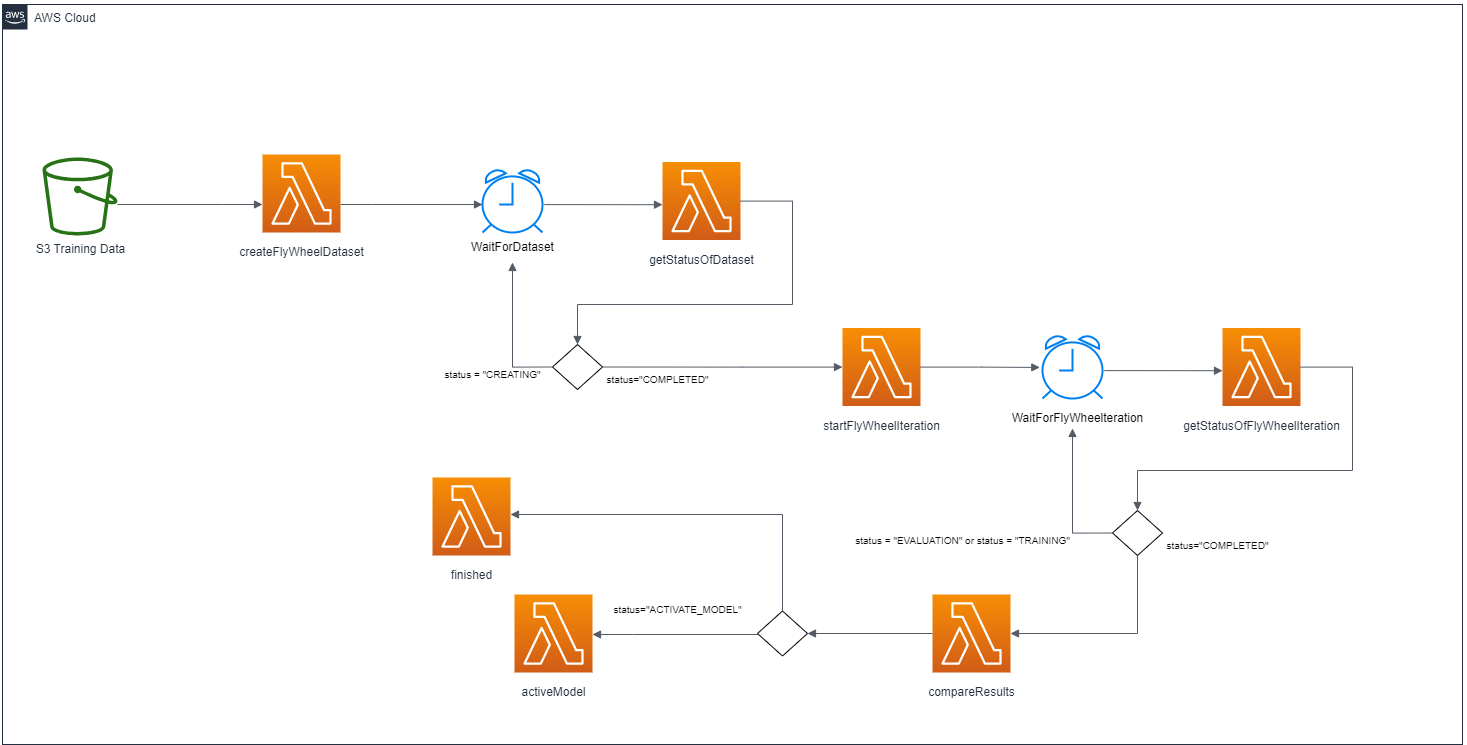
\includegraphics[width=1\textwidth]{img/active_learning_workflow.png}
  \caption{Active learning workflow}
  \label{fig:active_learning_workflow}
\end{figure}
Le sottosezioni successive hanno lo scopo di fornire una panoramica generale su un esempio di active learning workflow per migliorare il modello di classificazione di Comprehend.
\subsubsection{StartStepFunction}
\begin{itemize}
  \item \textbf{Trigger}: L'esecuzione è innescata dalla presenza di un file CSV contenente i dati di training.
  \item Il file CSV viene suddiviso in due file separati: uno per il training e uno per il testing.
  \item Viene avviata la Step Function.
\end{itemize}

\subsubsection{StartCustomClassification}
\begin{itemize}
  \item Viene utilizzata la funzione \texttt{create\_document\_classifier} per creare un classificatore personalizzato.
\end{itemize}
Si attende un periodo di 10 secondi per consentire la creazione del classificatore.

\subsubsection{GetStatusClassifier}
\begin{itemize}
  \item Viene utilizzata la funzione \texttt{describe\_document\_classifier} per ottenere lo stato attuale del classificatore. Gli stati possibili includono \texttt{SUBMITTED}, \texttt{TRAINING}, e altri stati come \texttt{IN\_ERROR}, \texttt{TRAINED}, \texttt{DELETING}, e \texttt{CreateEndpoint}.
  \item Se la variabile \texttt{CurrentClassifierSSM} è impostata, viene restituito lo stato corrente del classificatore.
  \item Se la variabile \texttt{CurrentClassifierSSM} non è impostata:
  \begin{itemize}
    \item Se lo stato è \texttt{TRAINED}, vengono salvate le variabili \texttt{CurrentClassifierSSM}, \texttt{CurrentTrainingDataSSM}, \texttt{CurrentTestDataSSM}, \texttt{CurrentTestingTruthDataSSM} e viene restituito lo stato \texttt{CreateEndpoint}.
  \end{itemize}
\end{itemize}
Nel \textit{choice state}, viene verificato:
\begin{itemize}
  \item Se lo stato è \texttt{TRAINED}, si passa allo stato successivo \texttt{StartValidationTest}.
  \item Se lo stato è \texttt{CreateEndpoint}, si passa allo stato \texttt{StartCustomClassificationEndpointCreation}.
  \item In caso contrario, si attende per 10 secondi e si richiama \texttt{GetStatusClassifier}.
\end{itemize}

\subsubsection{StartValidationTest}
\begin{itemize}
  \item Viene utilizzato il classificatore passato come evento e quello fornito come parametro.
  \item Viene eseguita la funzione \texttt{start\_document\_classification\_job} su entrambi i modelli per classificare i dati di test.
  \item La risposta di entrambi i modelli viene stampata.
  \item Si passa allo stato successivo, trasmettendo l'ID di entrambi i job.
\end{itemize}
Si attende un periodo di 10 secondi per consentire la creazione dei job.

\subsubsection{GetStatusValidationTest}
\begin{itemize}
  \item Viene utilizzata la funzione \texttt{describe\_document\_classification\_job} per ottenere lo stato dei job dei due modelli. Gli stati possibili includono \texttt{COMPLETED}, \texttt{STOP\_REQUESTED}, e altri stati come \texttt{STOPPED}, \texttt{FAILED}.
\end{itemize}
Nel \textit{choice state}, si verifica se lo stato di entrambi i job è \texttt{COMPLETED}. In caso affermativo, si passa allo stato successivo; in caso contrario, si attende per 10 secondi e si richiama \texttt{GetStatusValidationTest}.

\subsubsection{ComputeTestResults}
\begin{itemize}
  \item Vengono scaricati i risultati dei due job (file .gz).
  \item I risultati vengono salvati nella tabella \texttt{TestResultTable} su DynamoDB.
  \item Viene creata una matrice di confusione basata sui risultati e calcolati i parametri di \textit{precision}, \textit{recall}, e \textit{f1-score}.
  \item I parametri vengono salvati nella tabella \texttt{TestResultTable}.
  \item Viene effettuato un confronto su un parametro selezionato:
  \begin{itemize}
    \item Se il vecchio modello risulta migliore, viene restituito lo stato \texttt{DONT\_CREATE}.
    \item In caso contrario, vengono aggiornate le variabili \texttt{CurrentClassifierSSM}, \texttt{CurrentTrainingDataSSM}, \texttt{CurrentTestDataSSM}, \texttt{CurrentTestingTruthDataSSM} con i valori del nuovo modello e viene restituito lo stato \texttt{CREATE}.
  \end{itemize} 
\end{itemize}
Se lo stato è \texttt{DONT\_CREATE}, si passa alla lambda \texttt{FINISHED}; altrimenti, si procede alla lambda \texttt{StartCustomClassificationEndpointCreation}.

\section{Combinazione delle custom queries con analyze expense}
Si può combinare l'uso delle custom queries con analyze expense per migliorare l'estrazione delle informazioni associate a ordini e fatture. In particolare, si può confrontare la percentuale di correttezza delle informazioni estratte con l'uso di queste due funzionalità.

\section{Sviluppo di un'interfaccia grafica}
Invece di caricare manualmente gli allegati o le email nel bucket S3, è possibile sviluppare un'interfaccia grafica che consenta l'upload diretto degli allegati e delle email. Questa soluzione semplificherebbe il processo, migliorando l'efficienza e l'usabilità del sistema.

\section{Utilizzo di A2I (Amazon Augmented AI)}

Per migliorare la precisione del modello, è possibile utilizzare Amazon Augmented AI (A2I). Maggiori informazioni sono disponibili al seguente link: \href{https://aws.amazon.com/it/augmented-ai/}{Amazon Augmented AI}.

\section{Integrazione con un Sistema Documentale}

È possibile integrare il sistema con un sistema documentale per l'archiviazione delle email e degli allegati, migliorando la gestione e l'accessibilità dei documenti.

\section{Utilizzo di Amazon OpenSearch Service}

Amazon OpenSearch Service può essere utilizzato per l'indicizzazione delle informazioni in Amazon DynamoDB, facilitando la ricerca delle informazioni. Questo servizio offre un'esperienza di ricerca sicura e scalabile.

\section{Utilizzo di Amazon CloudFormation}

Amazon CloudFormation può essere utilizzato per automatizzare la creazione e la gestione delle risorse AWS, semplificando il processo di provisioning dell'infrastruttura.
    \chapter{Conclusioni}
\label{cap:conclusioni}
\emph{In questa sezione vengono presentate le conclusioni del lavoro svolto.}

% per avere termine di glossario con apice "g" che appare
Lorem \glsfirstoccur{\gls{sdkg}}
\\
% per avere termine di glossario normale
Lorem \gls{apig}

\section{Consuntivo finale}

Le ore di stage effettivamente svolte sono state 320, rispettando il monte ore previsto. Il lavoro svolto è stato suddiviso in diverse fasi, ognuna delle quali ha richiesto un impegno specifico. La fase iniziale di studio e formazione ha richiesto un tempo maggiore rispetto a quanto preventivato, in quanto ho dovuto approfondire le tecnologie e gli strumenti necessari per lo sviluppo del progetto. La fase di progettazione e sviluppo ha richiesto un impegno costante, ma sono riuscito a rispettare i tempi previsti. Infine, la fase di test e validazione ha richiesto un tempo inferiore rispetto a quanto preventivato, in quanto il prodotto sviluppato ha funzionato correttamente fin da subito.

\section{Raggiungimento degli obiettivi}
Gli obiettivi prefissati all'inizio del percorso (riportati nella sezione \ref{cap:descrizione-stage}) di stage sono stati raggiunti con successo. 

%\begin{UC}
%    \usecase
%\end{UC}

\section{Conoscenze acquisite}
TO DO

\section{Valutazione personale}
In conclusione, ritengo di essere soddisfatto del lavoro svolto e delle competenze acquisite durante il percorso di stage. L'esperienza ha rappresentato un'opportunità di crescita professionale e personale, permettendomi di mettermi alla prova in un contesto lavorativo reale e di confrontarmi con problematiche complesse. Ho potuto apprendere concetti relativi al cloud computing e all'applicazione di servizi cloud, oltre che un particolare approfondimento sulle tecnologie di machine learning per l'elaborazione intelligente dei documenti. Inoltre, ho avuto modo di lavorare in un team di sviluppo, migliorando le mie capacità di collaborazione e di comunicazione. Infine, ho potuto mettere in pratica le competenze acquisite durante il percorso di studi, dimostrando di saper affrontare con successo le sfide che mi sono state proposte.

    %% chktex-file 8
% chktex-file 44
% chktex-file 24
\chapter{Analisi dei requisiti}
\label{cap:analisi-requisiti}

\section{Casi d'uso}

Per lo studio dei casi di utilizzo del prodotto sono stati creati dei diagrammi.
I diagrammi dei casi d'uso (in inglese \emph{Use Case Diagram}) sono diagrammi di tipo \gls{uml} dedicati alla descrizione delle funzioni o servizi offerti da un sistema, così come sono percepiti e utilizzati dagli attori che interagiscono col sistema stesso.
Essendo il progetto finalizzato alla creazione di un tool per l'automazione di un processo, le interazioni da parte dell'utilizzatore devono essere ovviamente ridotte allo stretto necessario. Per questo motivo i diagrammi d'uso risultano semplici e in numero ridotto.

\begin{figure}[ht] 
    \centering 
    \includegraphics[width=0.7\columnwidth]{usecase/scenario-principale} 
    \caption{Use Case - UC0: Scenario principale}
\end{figure}

\begin{usecase}{0}{Scenario principale}
    \usecaseactors{Sviluppatore applicativi}
    \usecasepre{Lo sviluppatore è entrato nel plug-in di simulazione all'interno dell'IDE}
    \usecasedesc{La finestra di simulazione mette a disposizione i comandi per configurare, registrare o eseguire un test}
    \usecasepost{Il sistema è pronto per permettere una nuova interazione}
\label{uc:scenario-principale}
\end{usecase}

\begin{usecase}{1}{Gestione Utente}
    \usecaseactors{Amministratore, Utente Registrato}
    \usecasepre{L'utente deve essere autenticato nel sistema.}
    \usecasedesc{L'utente può gestire le informazioni del proprio profilo.}
    \usecasepost{Le modifiche vengono salvate nel sistema.}
    \usecasealt{Se l'utente non è autenticato, visualizza un messaggio di errore.}
\end{usecase}

\begin{usecase}{2}{Creazione Prodotto}
    \usecaseactors{Amministratore}
    \usecasepre{L'amministratore ha effettuato l'accesso al sistema.}
    \usecasedesc{L'amministratore può aggiungere un nuovo prodotto al catalogo.}
    \usecasepost{Il nuovo prodotto viene aggiunto con successo.}
    \usecasealt{Se i campi obbligatori non sono compilati, visualizza un messaggio di errore.}
\end{usecase}

\section{Requisiti}

Da un'attenta analisi dei requisiti e degli use case effettuata sul progetto è stata stilata la tabella che traccia i requisiti in rapporto agli use case.\\
Sono stati individuati diversi tipi di requisiti e si è quindi fatto utilizzo di un codice identificativo per distinguerli.\\
Il codice dei requisiti, dove ogni requisito è identificato con il carattere \textbf{R}, è così strutturato:

\begin{enumerate}
    \item[\textbf{F}:] Funzionale.
    \item[\textbf{Q}:] Qualitativo.
    \item[\textbf{V}:] Di vincolo.
    \item[\textbf{N}:] Obbligatorio (necessario).
    \item[\textbf{D}:] Desiderabile.
    \item[\textbf{Z}:] Opzionale.
\end{enumerate}

Nelle tabelle \ref{tab:requisiti-funzionali}, \ref{tab:requisiti-qualitativi} e \ref{tab:requisiti-vincolo} sono riassunti i requisiti e il loro tracciamento con gli use case delineati in fase di analisi.

\begin{table}[h]
\begin{tabularx}{\textwidth}{lXl}
\hline
    \textbf{Requisito} & \textbf{Descrizione} & \textbf{Use Case}\\
    \hline
    RFN-1 & L'interfaccia permette di configurare il tipo di sonde del test & UC1\\
\hline
\end{tabularx}
\vspace{4pt}
\caption{Tabella del tracciamento dei requisti funzionali}
\label{tab:requisiti-funzionali}
\end{table}

\begin{table}[h]
\begin{tabularx}{\textwidth}{lXl}
\hline
    \textbf{Requisito} & \textbf{Descrizione} & \textbf{Use Case}\\
    \hline
    RQD-1    & Le prestazioni del simulatore hardware deve garantire la giusta esecuzione dei test e non la generazione di falsi negativi & - \\
\hline
\end{tabularx}
\vspace{4pt}
\caption{Tabella del tracciamento dei requisiti qualitativi}
\label{tab:requisiti-qualitativi}
\end{table}

\begin{table}[h]
\begin{tabularx}{\textwidth}{lXl}
\hline
    \textbf{Requisito} & \textbf{Descrizione} & \textbf{Use Case}\\
    \hline
    RVO-1    & La libreria per l'esecuzione dei test automatici deve essere riutilizzabile & - \\
\hline
\end{tabularx}
\vspace{4pt}
\caption{Tabella del tracciamento dei requisiti di vincolo}
\label{tab:requisiti-vincolo}
\end{table}

\section{Tracciamento dei requisiti}

    
    %% chktex-file 8
% chktex-file 24

\chapter{Verifica e validazione}
\label{cap:verifica-validazione}

\begin{figure}[h!]
    \centering
    \includegraphics[width=1\columnwidth]{img/quantum_superposition.png}
    \caption{Lorem}
    \label{fig:enter-label}
\end{figure}

\lipsum[1-2]
    %% chktex-file 2
% chktex-file 24

\chapter{Processi e metodologie}
\label{cap:processi-metodologie}

Lorem ipsum dolor sit amet, consectetuer adipiscing elit. Aenean commodo ligula eget dolor. Aenean massa. Cum sociis natoque penatibus et magnis dis parturient montes, nascetur ridiculus mus. Donec quam felis, ultricies nec, pellentesque eu, pretium quis, sem.
% \cite{article:spooky}

\begin{figure}[h]
    \centering
    \includegraphics[height=5cm]{img/qubit.png}
    \caption{Lorem}
    \label{fig:qubit}
\end{figure}

\lipsum[1]

\section{Processo sviluppo prodotto}

    \appendix
    \backmatter
    \printglossary[type=\acronymtype, title=Acronimi e abbreviazioni, toctitle=Acronimi e abbreviazioni]
    \printglossary[type=main, title=Glossario, toctitle=Glossario]
    \chapter{Bibliografia}
\label{cap:bibliography}
%\cleardoublepage

\nocite{*}

% Books bibliography
%\printbibliography[heading=subbibliography, title={Books}, type=book]

% Articles bibliography
%\printbibliography[heading=subbibliography, title={Articles}, type=article]

% Websites bibliography
\printbibliography[heading=subbibliography, title={Siti web consultati}, type=online]


    % Acronyms
\newacronym[description={\glslink{aig}{Artificial Intelligence}}]
{ai}{AI}{Artificial Intelligence}

\newacronym[description={\glslink{apig}{Application Programming Interface}}]
{api}{API}{Application Program Interface}

\newacronym[description={\glslink{awsg}{Amazon Web Services}}]
{aws}{AWS}{Amazon Web Services}

\newacronym[description={\glslink{erpg}{Enterprise Resource Planning}}]
{erp}{ERP}{Enterprise Resource Planning}

\newacronym[description={\glslink{ictg}{Information and Communication Technology}}]
{ict}{ICT}{Information and Communication Technology}

\newacronym[description={\glslink{idpg}{Intelligence Document Processing}}]
{idp}{IDP}{Intelligence Document Processing}

\newacronym[description={\glslink{mlg}{Machine Learning}}]
{ml}{ML}{Machine Learning}

\newacronym[description={\glslink{nlpg}{Natural Language Processing}}]
{nlp}{NLP}{Natural Language Processing}

\newacronym[description={\glslink{ocrg}{Optical Character Recognition}}]
{ocr}{OCR}{Optical Character Recognition}

\newacronym[description={\glslink{pecg}{Posta Elettronica Certificata}}]
{pec}{PEC}{Posta Elettronica Certificata}

\newacronym[description={\glslink{sdkg}{Software Development Kit}}]
{sdk}{SDK}{Software Development Kit}

\newacronym[description={\glslink{umlg}{Unified Modeling Language}}]
{uml}{UML}{Unified Modeling Language}

\newacronym[description={\glslink{bpmg}{Business Process Management}}]
{bpm}{BPM}{Business Process Management}

\newacronym[description={\glslink{cpqg}{Configure, Price, Quote}}]
{cpq}{CPQ}{Configure, Price, Quote}

\newacronym[description={\glslink{rpag}{Robotic Process Automation}}]
{rpa}{RPA}{Robotic Process Automation}

\newacronym[description={\glslink{llmg}{Large Language Model}}]
{llm}{LLM}{Large Language Model}

\newacronym[description={\glslink{mlopsg}{Machine Learning Operations}}]
{mlops}{MLOps}{Machine Learning Operations}

\newacronym[description={\glslink{ideg}{Integrated Development Environment}}]
{ide}{IDE}{Integrated Development Environment}

\newacronym[description={\glslink{fmg}{Foundation Models}}]
{fm}{FM}{Foundation Models}

\newacronym[description={\glslink{versioncontrolsystemg}{Version Control System}}]
{vcs}{VCS}{Version Control System}

% Glossary entries
\newglossaryentry{agileg}{
    name=\glslink{agileg}{Agile},
    text = Agile,
    sort = agile,
    description ={Nell'ambito dell'ingegneria del software con il termine Agile si intende un insieme di metodi di sviluppo del software basati su processi iterativi e incrementali, dove i requisiti e le soluzioni si evolvono attraverso la collaborazione tra team auto-organizzati e interfunzionali}
}

\newglossaryentry{aig}{
    name=\glslink{ai}{AI},
    text = AI,
    sort = ai,
    description = {Per artificial Intelligence (AI) si intende l'insieme di tecnologie e metodi che permettono ai computer di eseguire attività che richiedono intelligenza umana, come il riconoscimento di immagini, il riconoscimento vocale, la traduzione automatica, ecc}
}
% da mettere :
% idp e scalabilità
% Glossary entries
\newglossaryentry{apig} {
    name=\glslink{api}{API},
    text=API,
    sort=api,
    description={In informatica con il termine \emph{API} si indica ogni insieme di procedure disponibili al programmatore, di solito raggruppate a formare un set di strumenti specifici per l'espletamento di un determinato compito all'interno di un certo programma. La finalità è ottenere un'astrazione, di solito tra l'hardware e il programmatore o tra software a basso e quello ad alto livello semplificando così il lavoro di programmazione}
}

\newglossaryentry{awsg} {
    name=\glslink{aws}{AWS},
    text=AWS,
    sort=aws,
    description={Amazon Web Services (AWS) è una piattaforma di servizi cloud che offre potenza di calcolo, storage di database, distribuzione di contenuti e altre funzionalità per aiutare le imprese a scalare e crescere}
}

\newglossaryentry{ictg} {
    name=\glslink{ict}{ICT},
    text=ICT,
    sort=ict,
    description={Con il termine Information and Communication Technology (ICT) si intende l'insieme delle tecnologie informatiche e telematiche utilizzate per la gestione delle informazioni e la comunicazione}
}

\newglossaryentry{idpg}{
    name=\glslink{idp}{IDP},
    text=IDP,
    sort=idp,
    description={Con il termine Intelligence document processing (IDP) si intende l'insieme di tecnologie che permettono di estrarre informazioni da documenti cartacei o digitali, elaborarle e trasformarle in dati strutturati}
}

\newglossaryentry{mlg}{
    name=\glslink{ml}{ML},
    text=ML,
    sort=ml,
    description={Per Machine Learning (ML) si intende un insieme di tecniche e algoritmi che permettono ai computer di apprendere dai dati e di migliorare le prestazioni in base all'esperienza, senza essere esplicitamente programmati. Il machine learning si basa su modelli statistici e matematici che permettono di fare previsioni o decisioni in base ai dati analizzati}
}

\newglossaryentry{nlpg}{
    name=\glslink{nlp}{NLP},
    text=NLP,
    sort=nlp,
    description={Natural Language Processing (NLP) è un campo dell'intelligenza artificiale che si occupa di interazioni tra computer e linguaggio umano. L'obiettivo principale di NLP è consentire ai computer di comprendere, interpretare e generare il linguaggio umano in modo che possano effettivamente comunicare con gli esseri umani in modo naturale}
}

\newglossaryentry{ocrg} {
    name=\glslink{ocr}{OCR},
    text=OCR,
    sort = ocr,
    description = {Optical Character Recognition (OCR) è
    una tecnologia che permette di convertire diversi tipi di documenti cartacei o digitali in testo digitale, in modo che possano essere elaborati e analizzati da un computer}
}

\newglossaryentry{pecg} {
    name=\glslink{pec}{PEC},
    text=PEC,
    sort=pec,
    description={La \emph{Posta Elettronica Certificata} (PEC) è un servizio di posta elettronica che garantisce l'invio e la ricezione di messaggi di posta elettronica con valore legale equivalente a quello della raccomandata con avviso di ricevimento}
}

\newglossaryentry{repositoryg} {
    name=\glslink{repositoryg}{Repository},
    text = repository,
    sort=repository,
    description = {Con il termine repository si intende un ambiente di archiviazione centralizzato in cui vengono conservati e gestiti i file di un progetto software. Il repository consente di tenere traccia delle modifiche apportate ai file, di collaborare con altri sviluppatori e di mantenere una cronologia delle versioni del software
    }
}

\newglossaryentry{scalabilitàg}{
    name=\glslink{scalabilitàg}{Scalabilità},
    text=Scalabilità,
    sort=scalabilità,
    description={In informatica, la scalabilità è la capacità di un sistema di crescere in dimensioni e complessità in modo lineare o sub-lineare rispetto all'aumento del carico di lavoro}
}

\newglossaryentry{sdkg} {
    name=\glslink{sdk}{SDK},
    text=SDK,
    sort=sdk,
    description={Un Software Development Kit (SDK) è un insieme di strumenti e librerie di sviluppo software che consentono ai programmatori di creare applicazioni per una piattaforma specifica, come un sistema operativo, un framework o un servizio cloud}
}

\newglossaryentry{scrumg}{
    name=\glslink{scrumg}{Scrum},
    text=Scrum,
    sort=scrum,
    description={In ingegneria del software, per Scrum si intende un framework agile per la gestione del ciclo di sviluppo del software. Scrum è caratterizzato da un approccio iterativo e incrementale, in cui il lavoro è organizzato in sprints di durata fissa, di solito di 2-4 settimane. Scrum prevede un team auto-organizzato e interfunzionale, che lavora in modo collaborativo per raggiungere gli obiettivi prefissati}
}

\newglossaryentry{umlg} {
    name=\glslink{uml}{UML},
    text=UML,
    sort=uml,
    description={In ingegneria del software \emph{Unified Modeling Language} (ing. linguaggio di modellazione unificato) è un linguaggio di modellazione e specifica basato sul paradigma object-oriented. L'\emph{UML} svolge un'importantissima funzione di ``lingua franca'' nella comunità della progettazione e programmazione a oggetti. Gran parte della letteratura di settore usa tale linguaggio per descrivere soluzioni analitiche e progettuali in modo sintetico e comprensibile a un vasto pubblico}
}

\newglossaryentry{serverlessg}{
    name=\glslink{serverlessg}{Serverless},
    text=serverless,
    sort=serverless,
    description={Per serverless si intende un modello di cloud computing in cui il fornitore di servizi cloud gestisce l'infrastruttura del server e le risorse di calcolo, e il cliente paga solo per il tempo di esecuzione delle funzioni. Il modello serverless consente di ridurre i costi e semplificare la gestione delle risorse, in quanto il cliente non deve preoccuparsi di configurare e mantenere i server}
}

\newglossaryentry{biasg}{
    name=\glslink{biasg}{Bias},
    text=bias,
    sort=bias,
    description={Nell'ambito del machine learning per bias si intende il fenomeno per cui un modello di machine learning è incline a fare previsioni errate a causa di dati di addestramento non rappresentativi o di un'architettura del modello sbagliata. Il bias può portare a discriminazioni e disuguaglianze, e può essere ridotto attraverso la raccolta di dati più rappresentativi e l'ottimizzazione dell'architettura del modello}
}

\newglossaryentry{activelearningg}{
    name=\glslink{activelearningg}{Active learning},
    text=active learning,
    sort=active learning,
    description={Nell'ambito del machine learning per active learning si intende una tecnica di apprendimento supervisionato in cui il modello di machine learning è in grado di selezionare autonomamente i campioni di addestramento più informativi da un pool di dati non etichettati. L'active learning consente di ridurre il costo dell'etichettatura dei dati e di migliorare le prestazioni del modello}
}

\newglossaryentry{bucketg}{
    name=\glslink{bucketg}{Bucket},
    text=bucket,
    sort=bucket,
    description={Nel contesto di AWS, per bucket si intende un contenitore di oggetti che consente di archiviare e organizzare i dati in Amazon S3. Un bucket può contenere un numero illimitato di oggetti e può essere configurato con diverse opzioni di accesso e sicurezza}
}

\newglossaryentry{erpg}{
    name=\glslink{erpg}{ERP},
    text=ERP,
    sort=erp,
    description={Enterprise Resource Planning (ERP) è un sistema di gestione aziendale che integra e automatizza i processi aziendali, come la contabilità, la gestione delle risorse umane, la produzione, la logistica, le vendite e il marketing. Un sistema ERP consente di migliorare l'efficienza, la produttività e la collaborazione all'interno dell'azienda}
}

\newglossaryentry{dataprotectiong}{
    name=\glslink{dataprotectiong}{Data protection},
    text=Data Protection,
    sort=data protection,
    description={Misure tecniche e organizzative che proteggono i dati personali e aziendali da accessi non autorizzati, modifiche, divulgazioni o distruzioni.}
}

\newglossaryentry{cybersecurityg}{
    name=\glslink{cybersecurityg}{Cybersecurity},
    text=Cybersecurity,
    sort=cybersecurity,
    description={La cybersecurity è l'insieme di pratiche e tecnologie utilizzate per proteggere sistemi, reti e dati da attacchi informatici, accessi non autorizzati, e altre minacce digitali.}
}

\newglossaryentry{ibmpowerg}{
    name=\glslink{ibmpowerg}{IBM Power},
    text=IBM Power,
    sort=ibm power,
    description={IBM Power Systems sono una famiglia di server e processori sviluppati da IBM utilizzati in ambienti aziendali per applicazioni critiche}
}

\newglossaryentry{gdpr}{
    name=\glslink{gdpr}{GDPR},
    text=GDPR,
    sort=gdpr,
    description={Il Regolamento Generale sulla Protezione dei Dati (GDPR) è una legge sulla privacy che regola la protezione dei dati personali dei cittadini dell'Unione Europea. Il GDPR è entrato in vigore il 25 maggio 2018 e stabilisce regole chiare per la raccolta, l'elaborazione e la conservazione dei dati personali}
}

\newglossaryentry{businessintelligenceg}{
    name=\glslink{businessintelligenceg}{Business Intelligence},
    text=Business Intelligence,
    sort=business intelligence,
    description={La Business Intelligence (BI) è un insieme di processi, strumenti e tecnologie che consentono alle aziende di raccogliere, analizzare e presentare informazioni aziendali per supportare la presa di decisioni informate. La BI si basa sull'analisi dei dati storici e in tempo reale per identificare tendenze, modelli e opportunità di business}
}

\newglossaryentry{performancemanagementg}{
    name=\glslink{performancemanagementg}{Performance Management},
    text=Performance Management,
    sort=performance management,
    description={Il Performance Management è un processo continuo di pianificazione, monitoraggio e valutazione delle prestazioni dei dipendenti per garantire che raggiungano gli obiettivi aziendali. Il Performance Management coinvolge la definizione degli obiettivi, la valutazione delle prestazioni, il feedback e lo sviluppo delle competenze}
}

\newglossaryentry{customerintelligenceg}{
    name=\glslink{customerintelligenceg}{Customer Intelligence},
    text=Customer Intelligence,
    sort=customer intelligence,
    description={La Customer Intelligence è l'insieme di processi, strumenti e tecnologie che consentono alle aziende di raccogliere, analizzare e utilizzare informazioni sui clienti per migliorare la customer experience, aumentare la fedeltà dei clienti e massimizzare il valore del cliente}
}

\newglossaryentry{governanceaziendaleg}
{
    name=\glslink{governanceaziendaleg}{Governance aziendale},
    text=Governance aziendale,
    sort=governance aziendale,
    description={La governance aziendale è il sistema di regole, processi e pratiche che guidano e controllano le attività e le decisioni all'interno di un'azienda. La governance aziendale si occupa di definire gli obiettivi, le politiche e le procedure dell'azienda, di monitorare le prestazioni e di garantire la conformità alle normative e agli standard}
}

\newglossaryentry{bpmg}{
    name=\glslink{bpmg}{BPM},
    text=BPM,
    sort=bpm,
    description={Il Business Process Management (BPM) è un approccio sistemico alla gestione dei processi aziendali che mira a migliorare l'efficienza, la qualità e l'agilità dell'azienda. Il BPM coinvolge l'analisi, la progettazione, l'automazione e il monitoraggio dei processi aziendali per garantire che siano allineati agli obiettivi aziendali e alle esigenze dei clienti}
}

\newglossaryentry{cpqg}{
    name=\glslink{cpqg}{CPQ},
    text=CPQ,
    sort=cpq,
    description={Il Configure, Price, Quote (CPQ) è un processo aziendale che consente alle aziende di configurare, quotare e vendere prodotti e servizi in modo rapido, accurato e redditizio. Il CPQ coinvolge la configurazione dei prodotti, la determinazione dei prezzi e la generazione di preventivi personalizzati per i clienti}
}

\newglossaryentry{rpag}{
    name=\glslink{rpag}{RPA},
    text=RPA,
    sort=rpa,
    description={La Robotic Process Automation (RPA) è una tecnologia che consente di automatizzare i processi aziendali ripetitivi e basati su regole utilizzando software robot. I robot software possono eseguire attività manuali, ripetitive e noiose in modo rapido, accurato e senza errori}
}

\newglossaryentry{llmg}{
    name=\glslink{llm}{LLM},
    text=LLM,
    sort=llm,
    description={Un Large Language Model (LLM) è un modello di linguaggio basato su reti neurali profonde che è stato addestrato su un vasto corpus di testo per generare testo naturale in modo coerente e convincente. Gli LLM sono utilizzati in applicazioni di generazione di testo, traduzione automatica, riassunto automatico e altre applicazioni di elaborazione del linguaggio naturale}
}

\newglossaryentry{generativeaig}{
    name=\glslink{generativeaig}{Generative AI},
    text=Generative AI,
    sort=generative ai,
    description={La Generative AI è un'area dell'intelligenza artificiale che si occupa di creare nuovi contenuti, come immagini, testo, musica e video, utilizzando modelli di machine learning generativi. La Generative AI è utilizzata in applicazioni di creazione di contenuti, design assistito da computer, e generazione di arte e musica}
}

\newglossaryentry{mlopsg}{
    name=\glslink{mlopsg}{MLOps},
    text=MLOps,
    sort=mlops,
    description={MLOps è una pratica che combina i principi e le pratiche dell'ingegneria del software con quelli del machine learning per creare, implementare e gestire modelli di machine learning in modo efficiente ed efficace. MLOps coinvolge la collaborazione tra team di sviluppo, data science e operazioni per garantire che i modelli di machine learning siano scalabili, affidabili e sicuri}
}

\newglossaryentry{deeplearningg}{
    name=\glslink{deeplearningg}{Deep Learning},
    text=Deep Learning,
    sort=deep learning,
    description={Il Deep Learning è un'area dell'intelligenza artificiale che si occupa di creare modelli di machine learning basati su reti neurali profonde. Il Deep Learning è utilizzato in applicazioni di riconoscimento di immagini, riconoscimento vocale, traduzione automatica e altre applicazioni di elaborazione del linguaggio naturale}
}

\newglossaryentry{computervisiong}
{
    name=\glslink{computervisiong}{Computer Vision},
    text=Computer Vision,
    sort=computer vision,
    description={La Computer Vision è un'area dell'intelligenza artificiale che si occupa di creare sistemi che possono interpretare e comprendere le immagini e i video in modo simile agli esseri umani. La Computer Vision è utilizzata in applicazioni di riconoscimento facciale, riconoscimento di oggetti, veicoli autonomi e altre applicazioni di visione artificiale}
}

\newglossaryentry{nosqlg}{
    name=\glslink{nosqlg}{NoSQL},
    text=NoSQL,
    sort=nosql,
    description={Il NoSQL è un'approccio alla gestione dei dati che si basa su modelli di dati non relazionali, come i database di documenti, i database di colonne, i database di grafi e i database chiave-valore. Il NoSQL è utilizzato per gestire grandi volumi di dati non strutturati e semi-strutturati in modo flessibile ed efficiente}
}

\newglossaryentry{ideg}{
    name=\glslink{ideg}{IDE},
    text=IDE,
    sort=ide,
    description={Un Integrated Development Environment (IDE) è un software che fornisce un ambiente integrato per lo sviluppo di software, comprensivo di editor di codice, compilatore, debugger e altre funzionalità di sviluppo. Un IDE semplifica il processo di sviluppo del software e aumenta la produttività dei programmatori}
}

\newglossaryentry{fmg}{
    name=\glslink{fm}{FM},
    text=FM,
    sort=fm,
    description={I Foundation Models (FM) sono modelli di linguaggio basati su reti neurali profonde che sono stati addestrati su un vasto corpus di testo per generare testo naturale in modo coerente e convincente. I FM sono utilizzati in applicazioni di generazione di testo, traduzione automatica, riassunto automatico e altre applicazioni di elaborazione del linguaggio naturale}
}

\newglossaryentry{versioncontrolsystemg}{
    name=\glslink{versioncontrolsystemg}{Version Control System},
    text=Version Control System,
    sort=version control system,
    description={Un Version Control System (VCS) è un sistema che registra le modifiche apportate ai file di un progetto software nel tempo, in modo che sia possibile ripristinare versioni precedenti, confrontare le modifiche e collaborare con altri sviluppatori. I VCS sono utilizzati per tenere traccia delle modifiche al codice sorgente e coordinare il lavoro di sviluppo}
}

\newglossaryentry{datasetg}{
    name=\glslink{datasetg}{Dataset},
    text=dataset,
    sort=dataset,
    description={Un dataset è un insieme di dati strutturati o non strutturati che vengono utilizzati per addestrare e valutare i modelli di machine learning. I dataset possono contenere dati di testo, immagini, audio, video o altri tipi di dati, e possono essere etichettati o non etichettati}
}
%\newglossaryentry{qiskitg} {
%name=\glslink{qiskit}{Qiskit},
%text=Qiskit,
%sort=qiskit,
%description={Qiskit ([quiss-kit] noun, software) %is an open-source SDK for working with quantum %computers at the level of extended quantum %circuits, operators, and primitives.}
%}

\end{document}